
\documentclass[conference]{IEEEtran}

\IEEEoverridecommandlockouts 
% this is needed to allow the \IEEEpubid command used to add the copyright
% notice at the bottom of the first page. 
% See  How_to_add_Copyright_in_LaTeX_file.txt  for more info

% *** MISC UTILITY PACKAGES ***
%
% \usepackage{ifpdf}
% Heiko Oberdiek's ifpdf.sty is very useful if you need conditional
% compilation based on whether the output is pdf or dvi.
% usage:
% \ifpdf
%   % pdf code
% \else
%   % dvi code
% \fi
% The latest version of ifpdf.sty can be obtained from:
% http://www.ctan.org/tex-archive/macros/latex/contrib/oberdiek/
% Also, note that IEEEtran.cls V1.7 and later provides a builtin
% \ifCLASSINFOpdf conditional that works the same way.
% When switching from latex to pdflatex and vice-versa, the compiler may
% have to be run twice to clear warning/error messages.

% *** CITATION PACKAGES ***
%
%\usepackage{cite}
% cite.sty was written by Donald Arseneau
% V1.6 and later of IEEEtran pre-defines the format of the cite.sty package
% \cite{} output to follow that of IEEE. Loading the cite package will
% result in citation numbers being automatically sorted and properly
% "compressed/ranged". e.g., [1], [9], [2], [7], [5], [6] without using
% cite.sty will become [1], [2], [5]--[7], [9] using cite.sty. cite.sty's
% \cite will automatically add leading space, if needed. Use cite.sty's
% noadjust option (cite.sty V3.8 and later) if you want to turn this off.
% cite.sty is already installed on most LaTeX systems. Be sure and use
% version 4.0 (2003-05-27) and later if using hyperref.sty. cite.sty does
% not currently provide for hyperlinked citations.
% The latest version can be obtained at:
% http://www.ctan.org/tex-archive/macros/latex/contrib/cite/
% The documentation is contained in the cite.sty file itself.
\usepackage{mathptmx,graphicx}
\DeclareGraphicsExtensions{.pdf,.png}

% *** GRAPHICS RELATED PACKAGES ***
%
%\ifCLASSINFOpdf
%\usepackage[pdftex]{graphicx}
  % declare the path(s) where your graphic files are
  % \graphicspath{{../pdf/}{../jpeg/}}
  % and their extensions so you won't have to specify these with
  % every instance of \includegraphics
%\DeclareGraphicsExtensions{.pdf,.png,.jpeg}
%\else
  % or other class option (dvipsone, dvipdf, if not using dvips). graphicx
  % will default to the driver specified in the system graphics.cfg if no
  % driver is specified.
%\usepackage[dvips]{graphicx}
  % declare the path(s) where your graphic files are
  % \graphicspath{{../eps/}}
  % and their extensions so you won't have to specify these with
  % every instance of \includegraphics
%\DeclareGraphicsExtensions{.eps}
%\fi
% graphicx was written by David Carlisle and Sebastian Rahtz. It is
% required if you want graphics, photos, etc. graphicx.sty is already
% installed on most LaTeX systems. The latest version and documentation can
% be obtained at: 
% http://www.ctan.org/tex-archive/macros/latex/required/graphics/
% Another good source of documentation is "Using Imported Graphics in
% LaTeX2e" by Keith Reckdahl which can be found as epslatex.ps or
% epslatex.pdf at: http://www.ctan.org/tex-archive/info/
%
% latex, and pdflatex in dvi mode, support graphics in encapsulated
% postscript (.eps) format. pdflatex in pdf mode supports graphics
% in .pdf, .jpeg, .png and .mps (metapost) formats. Users should ensure
% that all non-photo figures use a vector format (.eps, .pdf, .mps) and
% not a bitmapped formats (.jpeg, .png). IEEE frowns on bitmapped formats
% which can result in "jaggedy"/blurry rendering of lines and letters as
% well as large increases in file sizes.
%
% You can find documentation about the pdfTeX application at:
% http://www.tug.org/applications/pdftex





% *** MATH PACKAGES ***
%
\usepackage[cmex10]{amsmath}
% A popular package from the American Mathematical Society that provides
% many useful and powerful commands for dealing with mathematics. If using
% it, be sure to load this package with the cmex10 option to ensure that
% only type 1 fonts will utilized at all point sizes. Without this option,
% it is possible that some math symbols, particularly those within
% footnotes, will be rendered in bitmap form which will result in a
% document that can not be IEEE Xplore compliant!
%
% Also, note that the amsmath package sets \interdisplaylinepenalty to 10000
% thus preventing page breaks from occurring within multiline equations. Use:
\interdisplaylinepenalty=2500
% after loading amsmath to restore such page breaks as IEEEtran.cls normally
% does. amsmath.sty is already installed on most LaTeX systems. The latest
% version and documentation can be obtained at:
% http://www.ctan.org/tex-archive/macros/latex/required/amslatex/math/





% *** SPECIALIZED LIST PACKAGES ***
%
%\usepackage{algorithmic}
% algorithmic.sty was written by Peter Williams and Rogerio Brito.
% This package provides an algorithmic environment fo describing algorithms.
% You can use the algorithmic environment in-text or within a figure
% environment to provide for a floating algorithm. Do NOT use the algorithm
% floating environment provided by algorithm.sty (by the same authors) or
% algorithm2e.sty (by Christophe Fiorio) as IEEE does not use dedicated
% algorithm float types and packages that provide these will not provide
% correct IEEE style captions. The latest version and documentation of
% algorithmic.sty can be obtained at:
% http://www.ctan.org/tex-archive/macros/latex/contrib/algorithms/
% There is also a support site at:
% http://algorithms.berlios.de/index.html
% Also of interest may be the (relatively newer and more customizable)
% algorithmicx.sty package by Szasz Janos:
% http://www.ctan.org/tex-archive/macros/latex/contrib/algorithmicx/




% *** ALIGNMENT PACKAGES ***
%
\usepackage{array}
% Frank Mittelbach's and David Carlisle's array.sty patches and improves
% the standard LaTeX2e array and tabular environments to provide better
% appearance and additional user controls. As the default LaTeX2e table
% generation code is lacking to the point of almost being broken with
% respect to the quality of the end results, all users are strongly
% advised to use an enhanced (at the very least that provided by array.sty)
% set of table tools. array.sty is already installed on most systems. The
% latest version and documentation can be obtained at:
% http://www.ctan.org/tex-archive/macros/latex/required/tools/


%\usepackage{mdwmath}
%\usepackage{mdwtab}
% Also highly recommended is Mark Wooding's extremely powerful MDW tools,
% especially mdwmath.sty and mdwtab.sty which are used to format equations
% and tables, respectively. The MDWtools set is already installed on most
% LaTeX systems. The lastest version and documentation is available at:
% http://www.ctan.org/tex-archive/macros/latex/contrib/mdwtools/


% IEEEtran contains the IEEEeqnarray family of commands that can be used to
% generate multiline equations as well as matrices, tables, etc., of high
% quality.


%\usepackage{eqparbox}
% Also of notable interest is Scott Pakin's eqparbox package for creating
% (automatically sized) equal width boxes - aka "natural width parboxes".
% Available at:
% http://www.ctan.org/tex-archive/macros/latex/contrib/eqparbox/





% *** SUBFIGURE PACKAGES ***
%\usepackage[tight,footnotesize]{subfigure}
% subfigure.sty was written by Steven Douglas Cochran. This package makes it
% easy to put subfigures in your figures. e.g., "Figure 1a and 1b". For IEEE
% work, it is a good idea to load it with the tight package option to reduce
% the amount of white space around the subfigures. subfigure.sty is already
% installed on most LaTeX systems. The latest version and documentation can
% be obtained at:
% http://www.ctan.org/tex-archive/obsolete/macros/latex/contrib/subfigure/
% subfigure.sty has been superceeded by subfig.sty.



%\usepackage[caption=false]{caption}
%\usepackage[font=footnotesize]{subfig}
% subfig.sty, also written by Steven Douglas Cochran, is the modern
% replacement for subfigure.sty. However, subfig.sty requires and
% automatically loads Axel Sommerfeldt's caption.sty which will override
% IEEEtran.cls handling of captions and this will result in nonIEEE style
% figure/table captions. To prevent this problem, be sure and preload
% caption.sty with its "caption=false" package option. This is will preserve
% IEEEtran.cls handing of captions. Version 1.3 (2005/06/28) and later 
% (recommended due to many improvements over 1.2) of subfig.sty supports
% the caption=false option directly:
%\usepackage[caption=false,font=footnotesize]{subfig}
%
% The latest version and documentation can be obtained at:
% http://www.ctan.org/tex-archive/macros/latex/contrib/subfig/
% The latest version and documentation of caption.sty can be obtained at:
% http://www.ctan.org/tex-archive/macros/latex/contrib/caption/




% *** FLOAT PACKAGES ***
%
%\usepackage{fixltx2e}
% fixltx2e, the successor to the earlier fix2col.sty, was written by
% Frank Mittelbach and David Carlisle. This package corrects a few problems
% in the LaTeX2e kernel, the most notable of which is that in current
% LaTeX2e releases, the ordering of single and double column floats is not
% guaranteed to be preserved. Thus, an unpatched LaTeX2e can allow a
% single column figure to be placed prior to an earlier double column
% figure. The latest version and documentation can be found at:
% http://www.ctan.org/tex-archive/macros/latex/base/



%\usepackage{stfloats}
% stfloats.sty was written by Sigitas Tolusis. This package gives LaTeX2e
% the ability to do double column floats at the bottom of the page as well
% as the top. (e.g., "\begin{figure*}[!b]" is not normally possible in
% LaTeX2e). It also provides a command:
%\fnbelowfloat
% to enable the placement of footnotes below bottom floats (the standard
% LaTeX2e kernel puts them above bottom floats). This is an invasive package
% which rewrites many portions of the LaTeX2e float routines. It may not work
% with other packages that modify the LaTeX2e float routines. The latest
% version and documentation can be obtained at:
% http://www.ctan.org/tex-archive/macros/latex/contrib/sttools/
% Documentation is contained in the stfloats.sty comments as well as in the
% presfull.pdf file. Do not use the stfloats baselinefloat ability as IEEE
% does not allow \baselineskip to stretch. Authors submitting work to the
% IEEE should note that IEEE rarely uses double column equations and
% that authors should try to avoid such use. Do not be tempted to use the
% cuted.sty or midfloat.sty packages (also by Sigitas Tolusis) as IEEE does
% not format its papers in such ways.





% *** PDF, URL AND HYPERLINK PACKAGES ***
%
%\usepackage{url}
% url.sty was written by Donald Arseneau. It provides better support for
% handling and breaking URLs. url.sty is already installed on most LaTeX
% systems. The latest version can be obtained at:
% http://www.ctan.org/tex-archive/macros/latex/contrib/misc/
% Read the url.sty source comments for usage information. Basically,
% \url{my_url_here}.





% *** Do not adjust lengths that control margins, column widths, etc. ***
% *** Do not use packages that alter fonts (such as pslatex).         ***
% There should be no need to do such things with IEEEtran.cls V1.6 and later.
% (Unless specifically asked to do so by the journal or conference you plan
% to submit to, of course. )


% correct bad hyphenation here
\hyphenation{trans-former core-less micro-controller}


\begin{document}
%
% paper title
% can use linebreaks \\ within to get better formatting as desired
\title{A modular ADC system for power data \\acquisition utilising coreless PCB transformers \\for power and signal isolation}
%
%
% author names and affiliations
% use a multiple column layout for up to three different
% affiliations
\author{\IEEEauthorblockN{Michael T. Carpenter and Mark A. H. Broadmeadow}
\IEEEauthorblockA{School of Electrical Engineering and Computer Science\\
Queensland University of Technology\\
Brisbane, Australia\\
Email: michael.carpenter@student.qut.edu.au}}

% conference papers do not typically use \thanks and this command
% is locked out in conference mode. If really needed, such as for
% the acknowledgment of grants, issue a \IEEEoverridecommandlockouts
% after \documentclass

% use for special paper notices
%\IEEEspecialpapernotice{(Invited Paper)}

% this creates the copyright notice at bottom of first page as required for IEEE

% MAHB - No copyright for AUPEC
%\IEEEpubid{978--1--4799--5776--7/14/\$31.00~\copyright~2014~IEEE}

% make the title area
\maketitle

% There's a lot of vertical space after the title, can it be reclaimed??

\begin{abstract}
%\boldmath
% Not sure about my use of future tense when describing the measurement module here...
Although current industrial energy meters offer high accuracy and reliability, they are typically expensive and low-bandwidth, making them poorly suited to a multi-sensor data collection scheme.  As a result, this paper proposes a measurement device that is highly modular and extendible, as well as being compact and low-cost.  To minimise cost, the device will make use of planar coreless PCB transformers in order to provide galvanic isolation of its inputs and outputs.  The data from the acquisition devices would then be concentrated by a central processor before integration with existing control systems and computer consoles.  \\
This paper focusses on the practical use of planar coreless PCB transformers, which will facilitate the module's isolated power, clock and data signal transfer.  Calculations necessary to design coreless PCB transformers, and circuits designed for the transformer's practical application in the measurement module are presented.  The transformer itself and each application circuit has been experimentally verified, with test data and conclusions made applicable to coreless PCB transformers in general.
\end{abstract}

% Do keywords go somewhere?

\IEEEpeerreviewmaketitle

\section{Introduction}
% I think my introduction = abbstract (or vice-versa), not sure if this is OK..
Currently, industrial energy users are limited to expensive and low-bandwidth energy usage data collection devices. Although such metering devices are well suited to high-accuracy, high-energy systems, they are poorly suited to modular, multi-sensor data collection schemes.  To facilitate industrial process refinement, fault detection and energy usage analysis, Queensland University of Technology researchers are currently developing an isolated, low-cost, high-bandwidth data acquisition module (herein referred to as a DAQM).  Data from the network of distributed measurement modules will be concentrated by a central processor (such as an FPGA), with a microcontroller facilitating the data logging and integration into existing control systems and computer consoles.

% MC Removed to save space
%Conventionally, a galvanically isolated power supply is designed using a transformer with magnetic core to provide isolation.  Although a proven, reliable technology capable of high efficiency and high power transfer, the transformer can be an expensive and bulky component, especially in applications where the output power is very low.
%\\
%For isolated data transfer, opto-couplers are a popular solution for many low- to moderate-frequency systems, however devices capable of reliable operation at more than a few megaertz are expensive.  A relatively new method of signal isolation, the digital isolator, can operate at up to many tens of megahertz, however with a typical price of several dollars per two-channel unit (in 1ku quantities), their application in a low-cost device (such is the data acquisition module) is limited.

Planar coreless PCB transformers are not a new idea, and considerable work has been published on their use in isolated gate drive circuits \cite{TangHuiFundamental}\cite{NaturallySoft}\cite{OptimalOperation}\cite{CorelessGateDrive}.  Although wireless charging systems for consumer electronics use a very similar concept, coreless PCB transformers have not seen significant use as a power and signal transfer device within commercial electronics.  Since a coreless PCB transformer's only cost is the PCB area it consumes, they are well suited for low-cost applications, and the use of standard PCB manufacturing processes makes their construction predictable and repeatable.
\\
This paper will focus primarily on the practical application of planar coreless PCB transformers as used for the module's isolated power, clock and data signal transfer.  Calculations necessary to design the coreless PCB transformers are presented, and practical circuits designed for the DAQM application, but applicable to coreless PCB transformers in general, are included.  The experimental validation section demonstrates the viability of the use of coreless PCB transformers (and associated circuitry) in the DAQM application, with test data and conclusions made applicable to coreless PCB transformer-based designs in general.

\section{Proposed modular data acquisition system}
The complete data acquisition system (figure \ref{fig:FullSystem}) comprises of several data acquisition modules (DAQMs), a data concentrator and filter FPGA, and a microcontroller attached to a PC, display and/or storage device.  
The DAQM's data conversion device is a commercial dual-input sigma-delta modulator IC, with appropriate external signal conditioning to allow voltage measurement via a resistor divider, and current measurement via a shunt or current transformer (CT).  This paper will refer to the data conversion side of the DAQM as the ``secondary'' side.  The primary side of the DAQM consists of the coreless PCB transformer driver and data recovery circuitry.  Isolated secondary-side power and the modulator's external clock signal is provided by a single planar coreless PCB transformer.  This is teamed with a smaller,  higher frequency coreless PCB transformer used to transfer measurement data from the modulator back to the host.  For the selected sigma-delta modulator, the clock frequency will be approximately 8MHz, resulting in a data output rate of $ f_{clock}/4 $ (voltage and current share one Manchester-encoded data stream) with a maximum input sampling rate of $ f_{clock}/12 $.
% MC REMOVED: (basically a repeat)
%Whilst considerable work has been presented regarding the use of planar coreless PCB transformers in power transfer and isolated gate drive circuits, such papers do not discuss a high-frequency data and power transfer application \cite{TangHuiFundamental}\cite{NaturallySoft}\cite{OptimalOperation}\cite{CorelessGateDrive}.  The planar coreless PCB transformer, along with the methods used to transfer power, clock and data signals, will be the focus of this paper.

\begin{figure}[t]
	\centering
	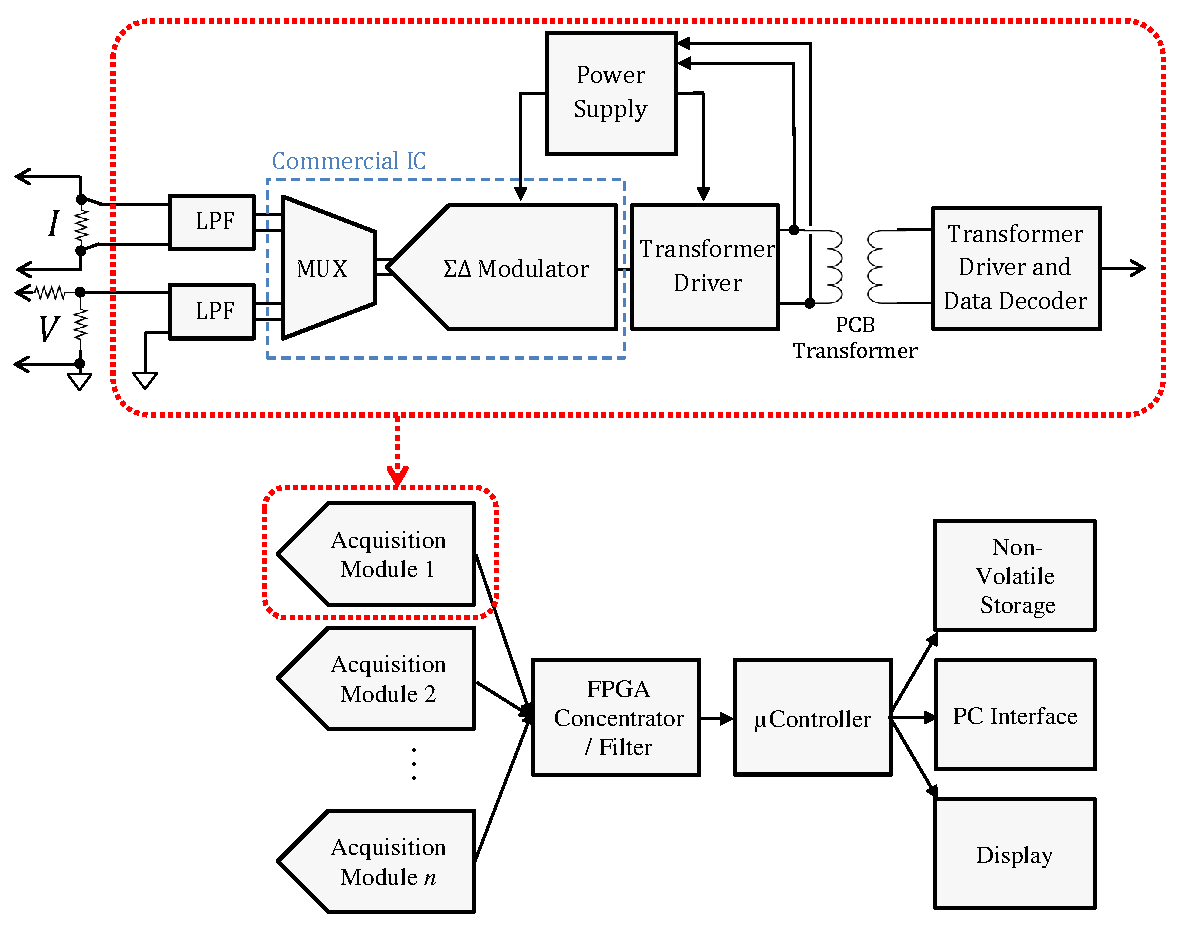
\includegraphics[width=1\columnwidth]{./img/FullSystem_BasicCol}
	\caption{Modular isolated power measurement system.}
	\label{fig:FullSystem}
\end{figure}

\section{Planar coreless PCB transformers}

The fundamental design of a planar coreless PCB transformer involves two planar copper spirals - one etched onto either side of a regular two or more layer PCB.  The two windings are thus separated by the PCB's core, whose material properties and thickness determine, to some extent, the transformer's performance and isolation voltage.  The transformer's primary winding is then driven at high frequency, usually in the range of 2MHz to 20MHz in order to achieve either the maximum [input] impedance frequency (MIF - for low power systems) or the maximum efficiency frequency (MEF - for high power systems)\cite{TangHuiFundamental}\cite{NaturallySoft}\cite{OptimalOperation}\cite{CorelessGateDrive}.  \cite{TangHuiFundamental} has demonstrated that an external secondary load capacitor, in the order of 100pF to 1nF, plays a significant role in the determination of the transformer's resonant frequency.  In conventional coreless PCB transformer applications, the output voltage is then rectified and filtered, and efficiencies exceeding 90\%, with a power density of up to $ 24W/cm^{2} $ have been demonstrated \cite{TangHuiFundamental}.

%Planar coreless PCB transformers are very low cost and feature high power densities, no manufacturing restrictions due to core size or shape and are constructed using highly repeatable standard PCB manufacturing process. 
%
\begin{figure}[t]
	\centering
	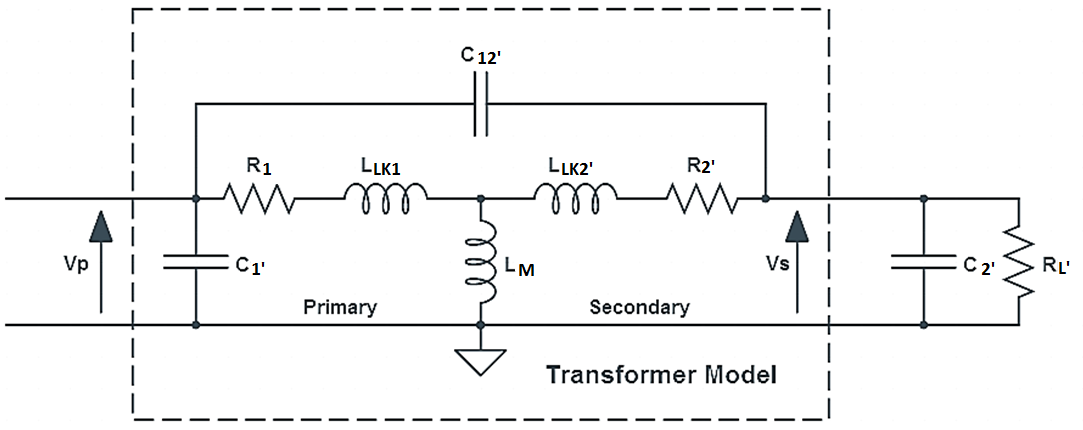
\includegraphics[width=1\columnwidth]{./img/HF_Model}
	\caption{High-frequency transformer model \cite{TangHuiFundamental}.}
	\label{fig:HF-Model}
\end{figure}

A two-winding coreless PCB transformer may be described using the high-frequency transformer model in figure \ref{fig:HF-Model} \cite{TangHuiFundamental}, where:
\begin{description}
\item[\hspace{-10pt}$ R_{1} $]    \hspace{-15pt} Primary winding resistance;
\item[\hspace{-10pt}$ R_{2}' $]   \hspace{-15pt} Secondary winding resistance, referred to primary;
\item[\hspace{-10pt}$ R_{L}' $]   \hspace{-15pt} Load resistance, referred to primary;
\item[\hspace{-10pt}$ L_{LK1} $]  \hspace{-15pt} Primary leakage inductance;
\item[\hspace{-10pt}$ L_{LK2}' $] \hspace{-15pt} Secondary leakage inductance, referred to primary;
\item[\hspace{-10pt}$ L_{M} $]    \hspace{-15pt} Mutual inductance;
\item[\hspace{-10pt}$ L_{p} $]    \hspace{-15pt} Primary self-inductance, equal to $ L_{M} + L_{LK1} $;
\item[\hspace{-10pt}$ L_{s} $]    \hspace{-15pt} Secondary self-inductance, equal to $ L_{M} + L_{LK2} $;
\item[\hspace{-10pt}$ C_{12} $]   \hspace{-15pt} Primary-to-secondary winding capacitance;
\item[\hspace{-10pt}$ C_{1} $]    \hspace{-15pt} Sum of primary winding capacitance and primary driver output capacitance;
\item[\hspace{-10pt}$ C_{2}' $]   \hspace{-15pt} Sum of secondary winding capacitance and external load capacitance, referred to primary;
\item[\hspace{-10pt}$ n $]        \hspace{-15pt} Turns ratio;
\item[\hspace{-10pt}$ \mu_{0} $]  \hspace{-15pt} Permeability of vacuum;
\item[\hspace{-10pt}$ a_{1} $]    \hspace{-15pt} Inner radius of $i$th circular track filament;
\item[\hspace{-10pt}$ a_{2} $]    \hspace{-15pt} Outer radius of $i$th circular track filament;
\item[\hspace{-10pt}$ h_{1} $]    \hspace{-15pt} Height of $i$th circular track filament;
\item[\hspace{-10pt}$ r_{1} $]    \hspace{-15pt} Inner radius of $j$th circular track filament;
\item[\hspace{-10pt}$ r_{2} $]    \hspace{-15pt} Outer radius of $j$th circular track filament;
\item[\hspace{-10pt}$ h_{2} $]    \hspace{-15pt} Height of $j$th circular track filament;
\item[\hspace{-10pt}$ z $]        \hspace{-15pt} Separation distance between the circular tracks;
\item[\hspace{-10pt}$ J_{0}(x) $] \hspace{-15pt} Bessel function of the first kind, order zero.
\end{description}
%
The self inductance of the planar winding \cite{HurleyDuffy} is given by
% PRI
\begin{equation}
	L_{p} = \sum\limits_{j=1}^{N_{p}}{\sum\limits_{i=1}^{N_{p}}{M_{ij}}}
\end{equation}
%
% SEC
\begin{equation}
	L_{s} = \sum\limits_{j=1}^{N_{s}}{\sum\limits_{i=1}^{N_{s}}{M_{ij}}}
\end{equation}
%
And thus, the mutual inductance between the two planar, multi-filament windings \cite{HurleyDuffy} may be represented as
%
\begin{equation}
	L_{M} = \sum\limits_{j=1}^{N_{p}}{\sum\limits_{i=1}^{N_{s}}{M_{ij}}}
\end{equation}
%
where the filament-to-filament mutual inductance, $ M_{ij} $, has been reported in \cite{HurleyDuffy}
% MAHB: Split equation over multiple lines
\begin{equation}
\begin{split}
	M_{ij} = \frac{\mu_{0}\pi}{h_{1}\ln(\frac{r_{2}}{r_{1}})h_{2}\ln(\frac{a_{2}}{a_{1}})}\int\limits_{0}^{\infty} & S(kr_{2},kr_{1})S(ka_{2},ka_{1}) 
	\\ &\quad {Q(kh_{1},kh_{2})e^{-k|z|}dk}
\end{split}
\end{equation}
%
where
\begin{equation}
	S(kx, ky) = \frac{J_{0}(kx) - J_{0}(ky)}{k}
\end{equation}
%
\begin{equation}
	Q(kx, ky) = \left\{
		\begin{array}{lr}
		\frac{2}{k^{2}} \left[ \cosh{k\frac{x+y}{2}}-\cosh{k\frac{x-y}{2}} \right] & z>\frac{h_{1}+h_{2}}{2} \\
		\frac{2}{k} \left[ h+\frac{e^{-kh}-1}{k} \right] & z=0, x=y=h
		\end{array}
   \right.
\end{equation}

\hspace{-15pt}Note that $z = 0$ for the calculation of self-inductances. 
To approximate the performance of the coreless PCB transformer, \cite{TangHuiFundamental} gives the resonant frequency as
%
\begin{equation}
	f_{0} = \frac{1}{2\pi\sqrt{L_{eq}C_{eq}}};
\end{equation}
%
and the $s$-domain voltage gain (\ref{eqn:vGain}) and input impedance (\ref{eqn:zIn}) as
%
\begin{equation}
	\label{eqn:vGain}
	\frac{V_{s}}{V_{p}} = G(s) = B = \frac{\frac{1}{X_{1}}+sC_{12}'Y_{1}}{nY};
\end{equation}
%
\begin{equation}
	\label{eqn:zIn}
	Z_{in} = \frac{1}{sC_{12}'(1-nB)+\frac{1-A}{X_{1}}+sC_{1}'}.
\end{equation}
%
Although not of great concern to the DAQM application (due to the low secondary power requirements), the coreless PCB transformer's efficiency  may be calculated as \cite{TangHuiFundamental}
% Power out
\begin{equation}
	P_{out} = \frac{|G(s)|^{2}\cdot|V_{p}|^{2}}{R_{L}};
\end{equation}
% Power in
\begin{equation}
	P_{in} = |V_{p}|^{2}\cdot\Re \left[ \frac{1}{Z_{in}} \right];
\end{equation}
and thus,
% Efficiency
\begin{equation}
	\eta = \frac{|G(s)|^{2}}{R_{L}\cdot\Re \left[ \frac{1}{Z_{in}} \right]}\times 100 \%.
\end{equation}
%
Where
%
\begin{align*}
	L_{eq}   &= L_{LK2}'+L_{LK1}||L_{M} 	\\
	C_{eq}   &= C_{2}'+C_{12}'				\\
	R_{2}'   &= n^{2}R_{2}					\\
	L_{LK2}' &= n^{2}L_{LK2}				\\
	C_{1}'   &= C_{1} + \frac{n-1}{n}C_{12}	\\
	C_{2}'   &= \frac{1}{n^{2}}C_{2} + \frac{1-n}{n^{2}}C_{12}	\\
	C_{12}'  &= \frac{1}{n}C_{12}			\\
	X_{1}    &= R_{1}  + sL_{LK1}			\\
	X_{2}    &= R_{2}' + sL_{LK2}'			\\
	Y_{1}    &= X_{2} \lbrack \frac{1}{X_{1}} + \frac{1}{sL_{M}} \rbrack +1	\\
	Y_{2}    &= \frac{1}{X_{2}} + sC_{12}' + sC_{2}' + \frac{1}{n^{2}R_{L}}	\\
	Y        &= -\frac{1}{X_{2}} + Y_{1}Y_{2}	\\
	A        &= \frac{sC_{12}' + \frac{X_{2}}{X_{1}} Y_{2}}{Y}
\end{align*}
%
\section{Implementation of power and signal isolation using PCB transformers}

	\subsection{Power}
	The most basic use for a planar coreless PCB transformer is in an isolated power transfer application.  Typically, this would be achieved by driving the transformer at its maximum efficiency frequency (MEF) for high power transfer applications, or, where it is desirable to minimise the quiescent power consumption of the transformer, the maximum impedance frequency (MIF).  The MEF will tend to approach the MIF as the transformer's secondary load current decreases \cite{TangHuiFundamental}.  
	Due to the low secondary load current of the DAQM - approximately 6mA at 3.3V (20mW), the MEF of the module's coreless PCB transformer was initially assumed to be equal to the MIF.  In most papers discussing planar coreless PCB transformers, the primary winding is driven in either a single-ended or bipolar manner (figure \ref{fig:BIvsSE}) with a relatively high supply voltage (12V being a popular choice for isolated gate drive circuits).  Since the DAQM is to be a 3.3V supply capable device, the PCB transformer was driven in a bipolar manner to achieve an effective doubling of the primary drive voltage.  The primary drive circuit uses a simple relaxation oscillator for the resonant frequency generation, and the transformer's winding is driven directly by the Schmitt-trigger's high-current (170mW at 85$ \,^{\circ} $C or $\pm$100mA maximum) push-pull outputs (figure \ref{fig:TFpwrclk}).
	On the transformer's secondary side, the output waveform may simply be rectified using a voltage-doubler rectifier topology \ref{fig:TFpwrclk}, with a zener clamping diode to ensure the voltage regulator's maximum input voltage is not exceeded.  The additional load capacitance, primarily due to the rectifier diode array D2 and coupling capacitor C4, may be estimated as the series coupling capacitor (C4) in parallel with the sum of the two diode junction capacitances in rectifier array D2.  For the rectifier circuit shown in figure \ref{fig:TFpwrclk}, the maximum additional capacitance is about 20pF, resulting in an expected resonant frequency shift of -10\%.
	
	\begin{figure}[t]
		\centering
		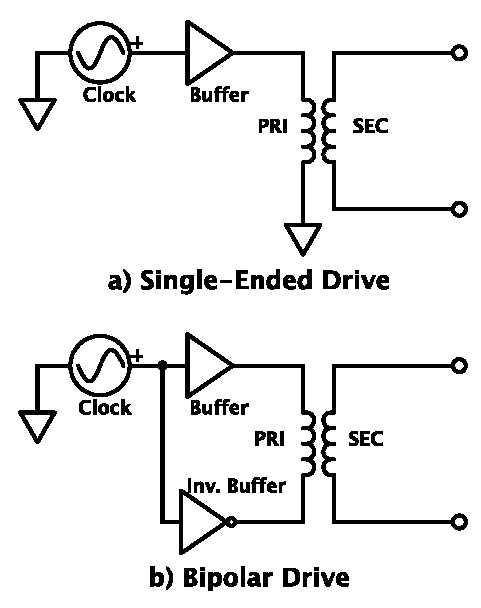
\includegraphics[width=0.9\columnwidth]{./img/BIvsSE}
		\caption{Single-ended (a) and bipolar (b) transformer drive concept.}
		\label{fig:BIvsSE}
	\end{figure}
%	
	\begin{figure*}[t]
		\centering
		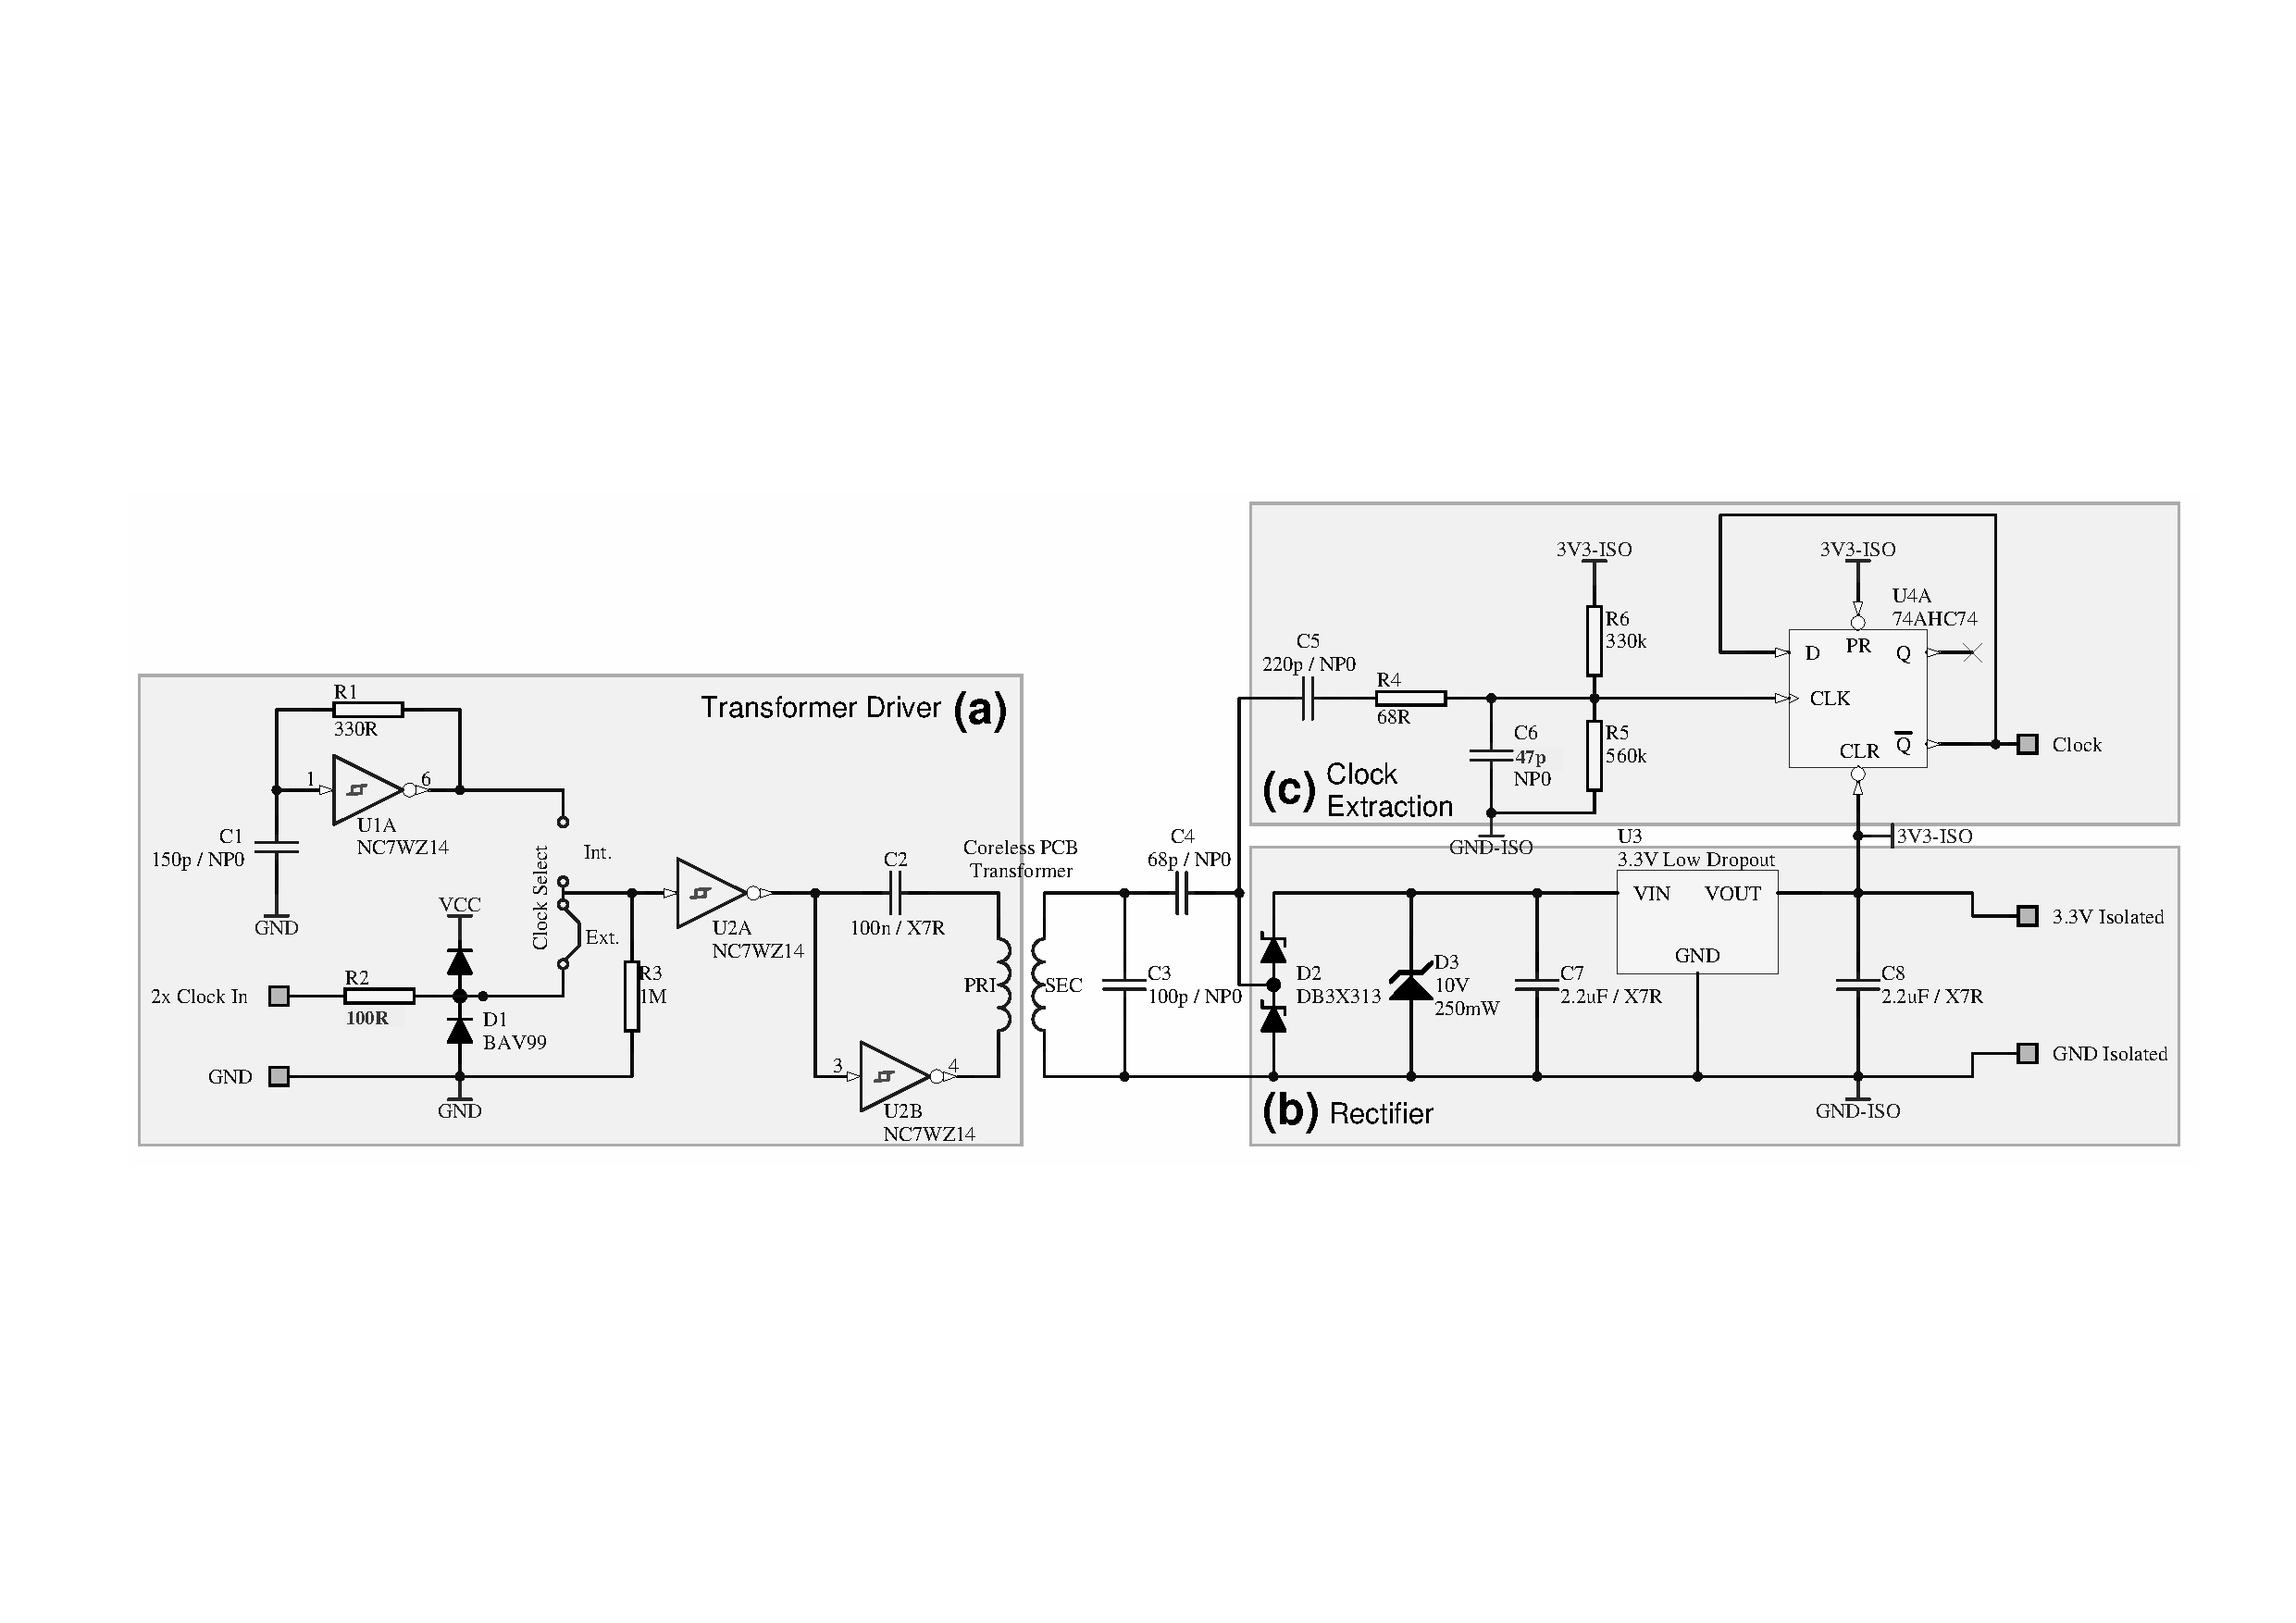
\includegraphics[width=1.0\textwidth]{./img/TFpwrclk_BW}
		\caption{Coreless PCB transformer driver (a) with power rectifier (b) and clock extraction circuitry (c) highlighted.}
		\label{fig:TFpwrclk}
	\end{figure*}	
	
	\subsection{Clock Generation and Recovery}
	In order to provide a clock signal of approximately 8MHz to the sigma-delta modulator, a method of transferring this clock signal (via the PCB transformer) from the DAQM's primary side to the secondary side was required.  It is desirable to allow the sigma-delta modulator to be externally clocked as this allows for synchronisation in multi-module systems, thus simplifying the filtering and data concentration process.  Since the clock frequency was to remain relatively fixed, the simplest method of transferring the signal to the DAQM's isolated side was to set the coreless PCB transformer's primary drive frequency to be equal to a power-of-two multiple of the desired clock frequency.  In this way, the clock signal could be extracted by rectifying, filtering and dividing the transformer's secondary voltage waveform (figure \ref{fig:TFpwrclk}).
	%Since a coreless PCB transformer's resonant frequency may be adjusted quickly and easily using the external load capacitance, it is possible to drive the transformer at any power-of-two multiple of the desired modulator clock frequency (provided the resulting drive frequency results in sufficient secondary output voltage).	
	
	\subsection{Data Recovery}
	% MC REMOVED: As the data frequency approaches the transformer's resonant frequency, the transformer's output voltage can be seen to 'ring' after the fundamental edge transition is transmitted - a benefit when maximum power transfer is required, but detrimental to the signal integrity of data transmissions.
	The sigma-delta modulator encodes both voltage and current information into a single Manchester-encoded bitstream at a rate equal to $ f_{clock}/4 $ (typically 2MHz).  To transfer this data back to the primary side of the data acquisition module, a second coreless PCB transformer was used.  Since the data signal is not periodic in the way that a clock signal is, it was necessary to configure the data transformer for a very high resonant frequency, thus ensuring that only the high-frequency square wave transitions were sent over the coil.  To achieve this, the equations in section `Planar coreless PCB transformers' imply that either the number of primary and secondary turns (and thus the primary and secondary winding outer diameter) should be decreased, and/or the external load capacitor may be reduced or removed. \\
	Figure \ref{fig:TFdat} shows the signal transformer and data recovery circuit.  On the coreless PCB transformer's secondary side, the data output of the modulator is capacitively coupled into the signal transformer, which is driven in a single-ended configuration.  On the primary side, the low-amplitude (50mV to 500mV may be expected) positive- and negative-going spikes, which represent the rising and falling edges of the data signal respectively, are first amplified by a bipolar junction transistor (BJT - Q1).  The amplifier's output is then coupled into two more BJTs with necessary biasing to allow the discrimination of the positive- and negative-going transitions (Q2 and Q3 respectively).  The output of each of the `edge transition detectors' is then fed into a set/reset latch constructed from a dual Schmitt-input NAND array to complete the decoding circuit.  As an added benefit, the outputs of the two NAND gates are complementary, thus allowing for differential signal driving back to the host FPGA (which may be located some distance away).
%
	\begin{figure}[t]
		\centering
		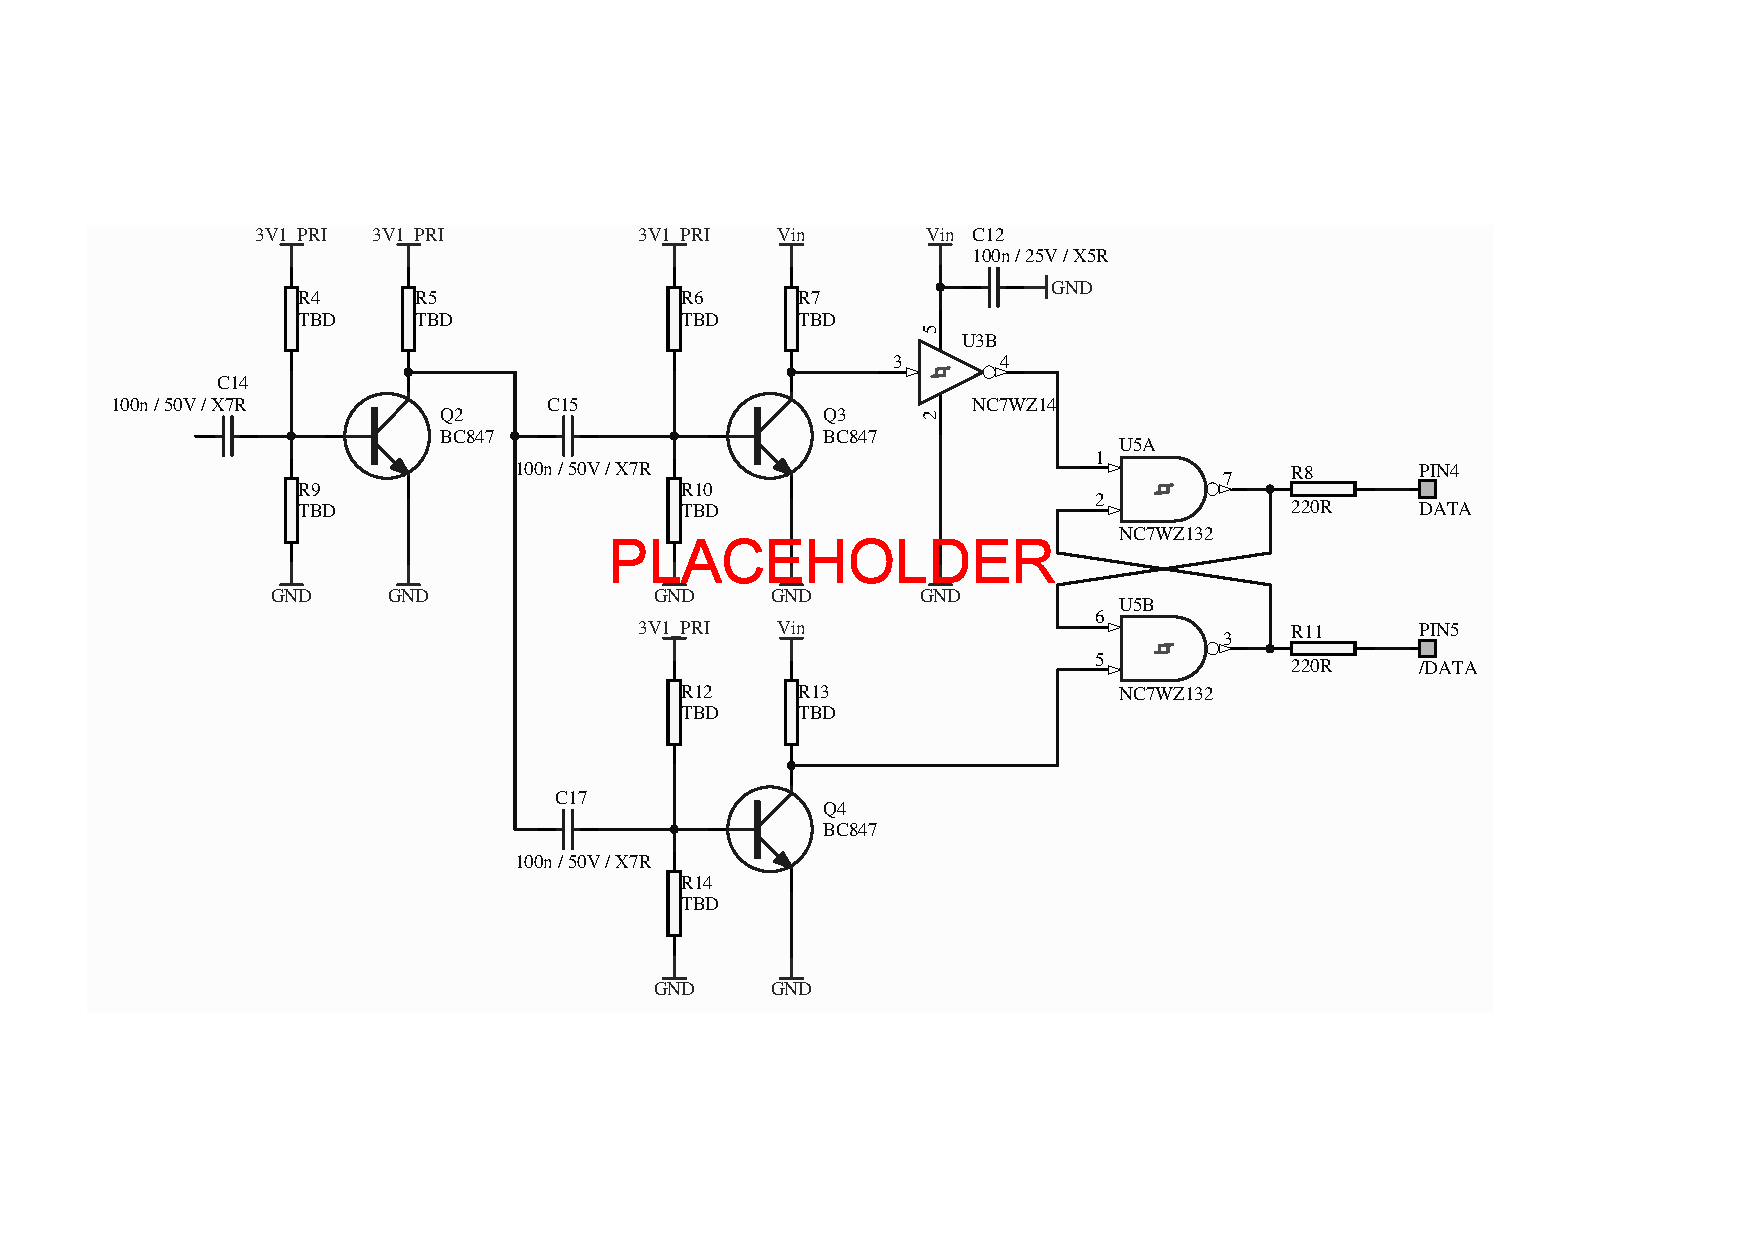
\includegraphics[width=1\columnwidth]{./img/TFdat_BW}
		\caption{Signal transformer and isolated data recovery circuit.}
		\label{fig:TFdat}
	\end{figure}
%	
\section{Experimental validation}
To validate the use of planar coreless PCB transformers in the data acquisition module design, a test PCB transformer was manufactured on a standard two-layer, 1.6mm PCB.  The test transformer had 11 turns with identical primary and secondary windings, a track and spacing width equal to $ 254\mu $m (10 mil), a 100pF external load capacitor (C3 in figure \ref{fig:TFpwrclk}) and a 500$\Omega$ load resistor.  With an outer diameter of 14mm and inner diameter of 2.8mm, the transformer's calculated and measured inductive parameters (200kHz test frequency) were:

% tablesgenerator.com
\begin{table}[h]
\begin{tabular}{l|l|l|l|}
\cline{2-4}
              & \textbf{Calculated} & \textbf{Measured} & \textbf{Error (\%)} \\[3pt] \hline 
\multicolumn{1}{|l|}{$\mathbf{L_{p}}$}   & 890.6nH    & 930nH    & 4.5\%      \\[3pt] \hline 
\multicolumn{1}{|l|}{$\mathbf{L_{LK1}}$} & 418.5nH    & 465nH    & 10\%       \\[3pt] \hline 
\multicolumn{1}{|l|}{$\mathbf{L_{s}}$}   & 890.6nH    & 930nH    & 4.5\%      \\[3pt] \hline 
\multicolumn{1}{|l|}{$\mathbf{L_{LK2}}$} & 418.5nH    & 465nH    & 10\%       \\[3pt] \hline 
\multicolumn{1}{|l|}{$\mathbf{L_{M}}$}   & 472.1nH    & 465nH    & -1.5\%     \\[3pt] \hline
\end{tabular}
\end{table}

Figure \ref{fig:NoRect} shows the test transformer's calculated and measured input impedance and voltage gain versus frequency, where only the secondary-side load resistor of 500$\Omega$ is fitted (that is, no rectifier or clock decoder).  The plots show a MEF (9dB voltage gain) at 18MHz and a MIF (142$\Omega$ input impedance) at about 14.5MHz (measured values).  The calculated performance curves are shown to be a good representation of the actual device performance, especially with regard to the coreless PCB transformer's voltage gain.
%
\begin{figure}[t]
	\centering
	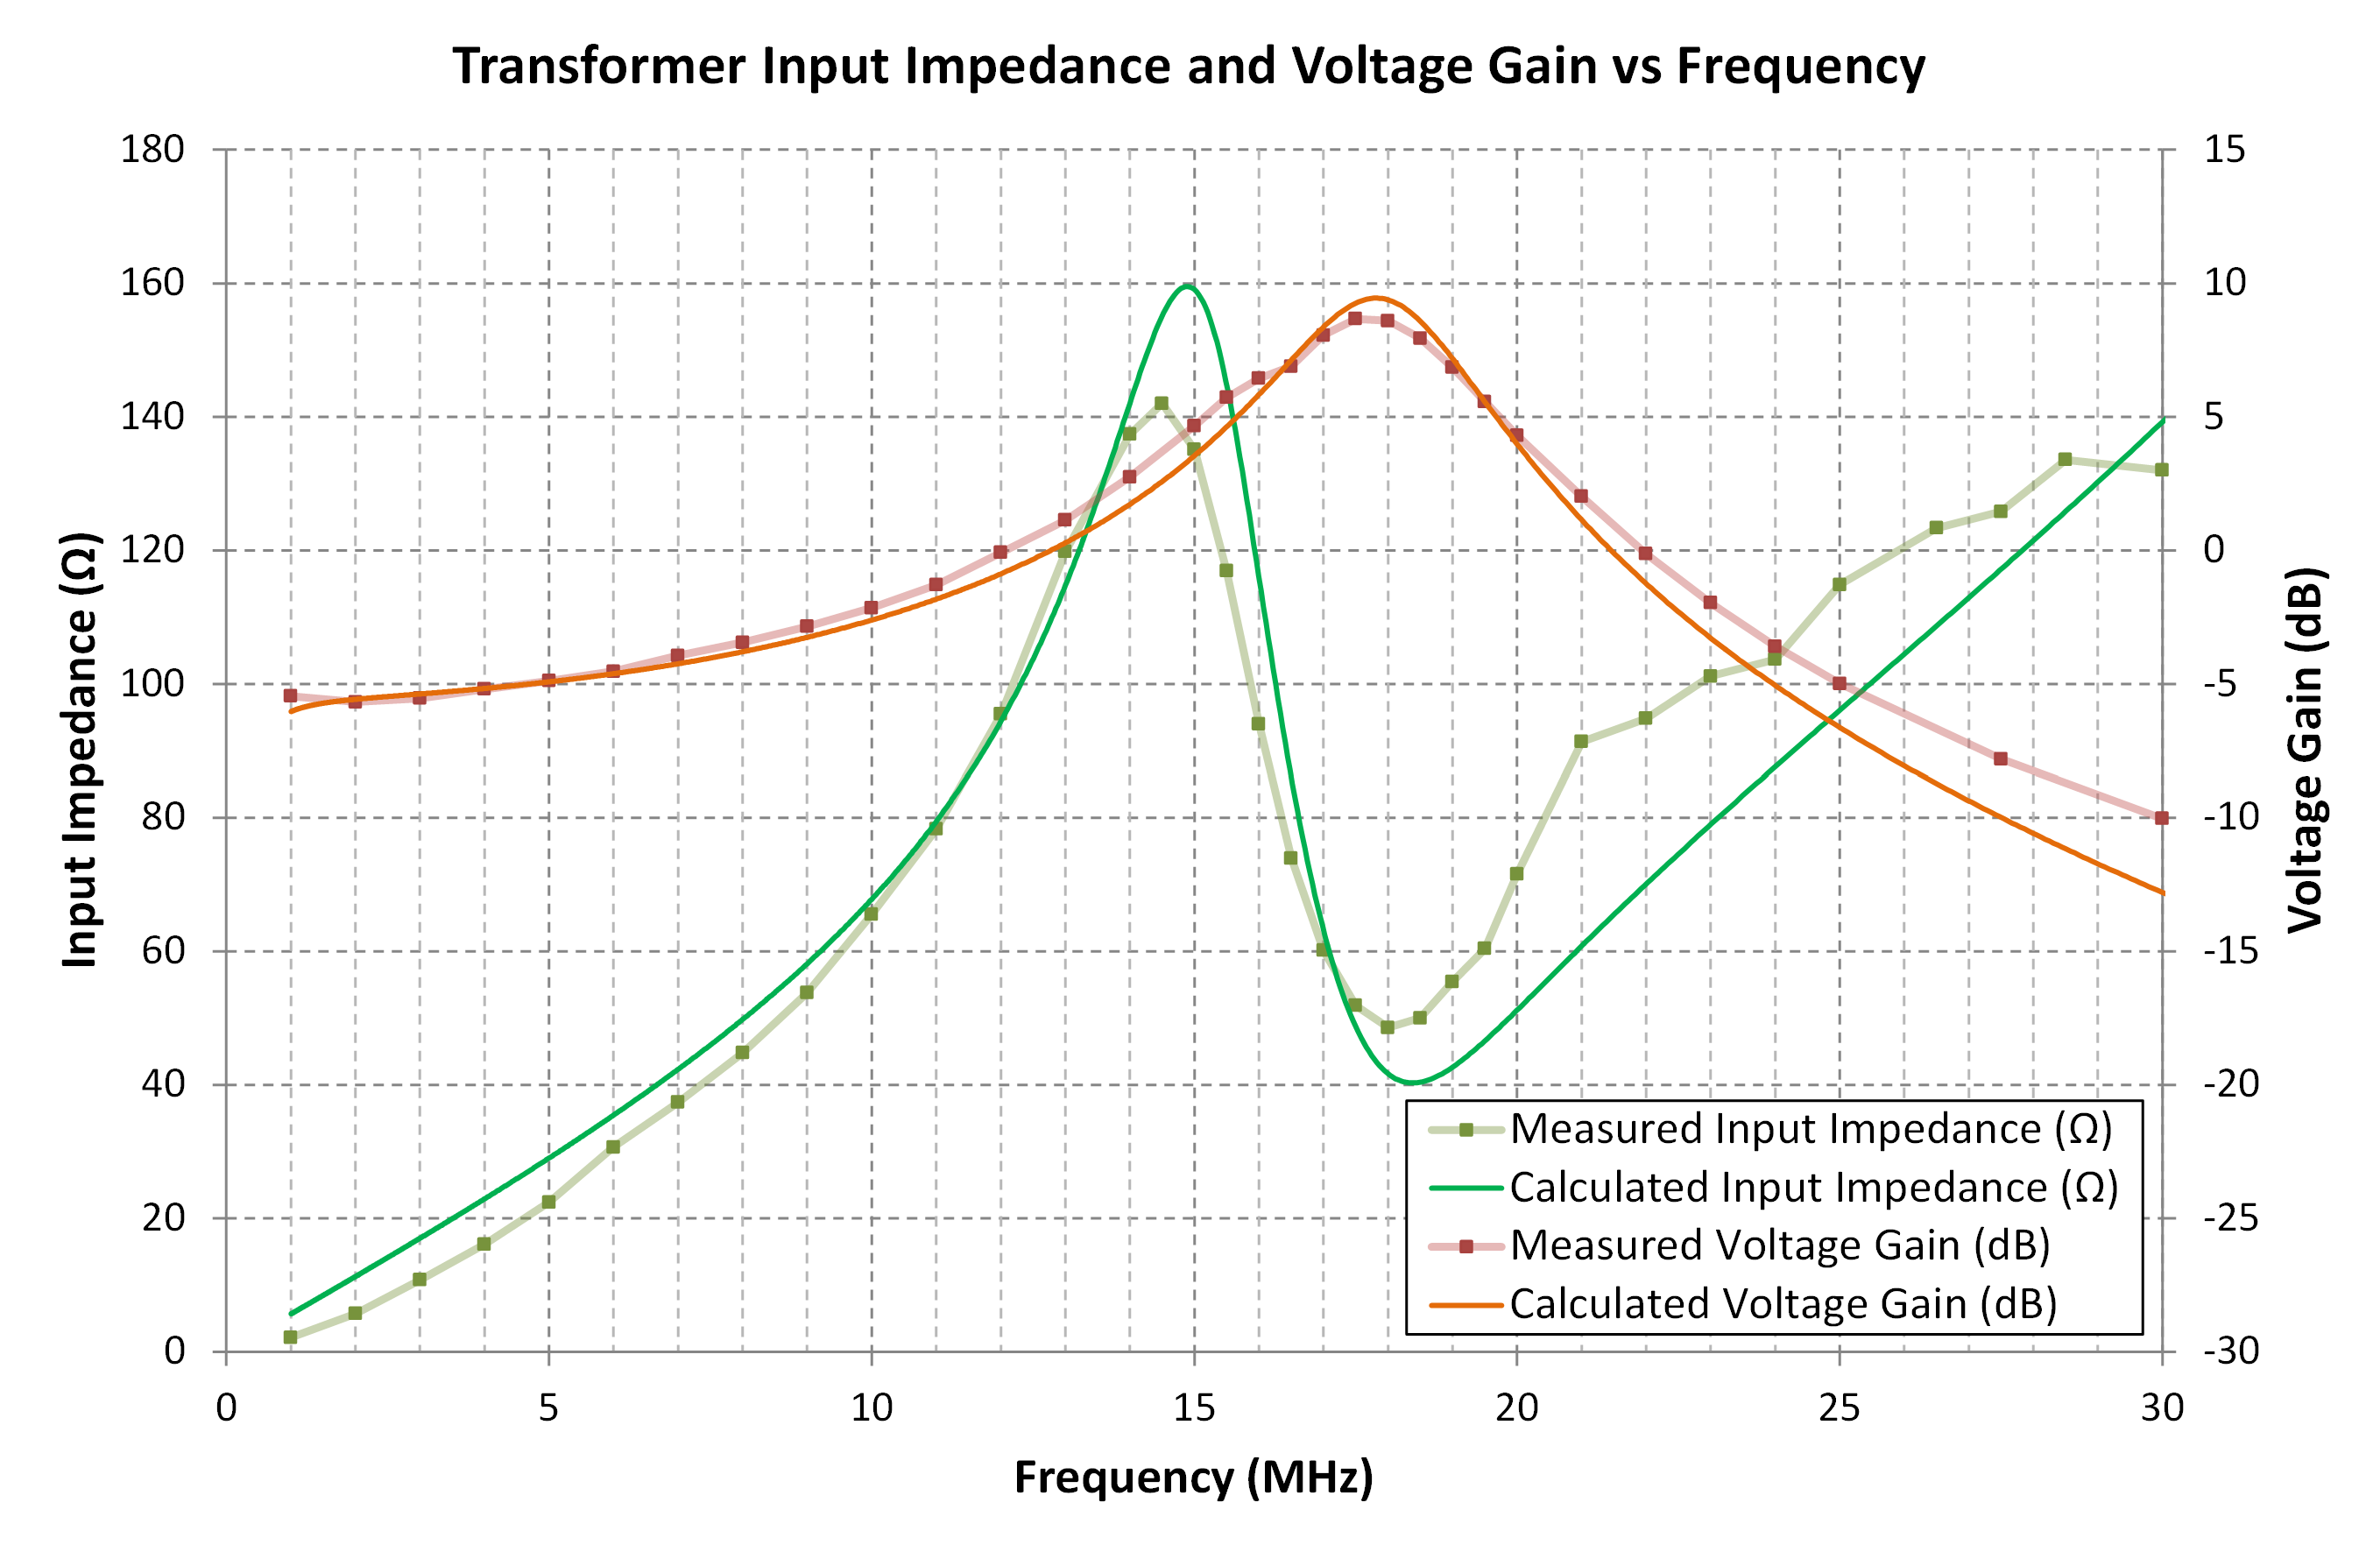
\includegraphics[width=1.0\columnwidth]{./img/NoRectTF}
	\caption{Test transformer's input impedance and voltage gain versus drive frequency.}
	\label{fig:NoRect}
\end{figure}
%
% Removed photograph to save space
%\begin{figure}[t]
%	\centering
%	\includegraphics[width=0.8\columnwidth]{./img/DAQMphoto}
%	\caption{Photograph of an initial unpopulated DAQM prototype with single 11-turn transformer.}
%	\label{fig:DAQMphoto}
%\end{figure}
%
	\subsection{Power}
	%To approximate the expected load of the sigma-delta modulator and associated secondary circuitry, a $500\Omega $ load resistor was fitted after the rectifier.  By sweeping the primary drive frequency over the range of 500kHz to 25MHz, the coreless PCB test transformer, with primary-side Schmitt trigger driver and secondary side rectifier could be analysed for input impedance- and output voltage- versus frequency (FIGURE).  
	With the rectifier (no regulator; 500$\Omega$ load resistor) and clock extraction circuitry (figure \ref{fig:TFpwrclk}) fitted, figure \ref{fig:ZandVvsF} shows the coreless PCB transformer's primary RMS drive current and rectifier output voltage versus frequency (at 3.3V drive voltage).  
	The figure shows a reduction in the maximum impedance and efficiency frequencies (14.5MHz and 18Mhz to 13MHz and 15.5MHz respectively), most likely due to the additional load capacitance presented by the rectifier diodes.  Whilst this frequency change can be predicted (as discussed prior) and accounted for by altering the load capacitor (C3 in figure \ref{fig:TFpwrclk}), in this case, the desired drive frequency is 16MHz and thus adjustment was not necessary.  \\
	The experimental data also demonstrates the effectiveness of driving the transformer in a bipolar manner, which has resulted in an output voltage approximately 1.6 times the 3.3V primary supply voltage - thus increasing the usable voltage range of the data acquisition module and simplifying the secondary voltage supply circuitry.  Additionally, the wide frequency range for which the output voltage is adequate for 3.3V regulation, may allow the transformer to be driven at a compromise frequency between the MIF and MEF in an effort to reduce primary drive current.
	
	Figure \ref{fig:VandPvsI} shows the coreless PCB test transformer's secondary rectified output power and voltage versus load current.  It shows a maximum power point of 47mW, and that for a minimum pre-regulator voltage of 3.5V, the load current may be up to 11mA (about 40mW) - twice the expected power required by the DAQM's secondary circuitry.  \\
	As a compromise between the MIF (13MHz) and MEF (15.5MHz), the test transformer drive frequency was adjusted to 14MHz (figure \ref{fig:VanndPvsI_retuned}).  This data shows improved load regulation and a shift in the maximum power point toward greater load currents, as well as a slight reduction in maximum power (approximately 40mW max versus 47mW max).  This suggests that transformer operation at a MIF-MEF compromise frequency (rather than at the MEF exactly) can have benefits for applications with relatively substantial secondary loads where the primary is driven by a current-limited source (such as the Schmitt trigger direct-drive circuit used in the DAQM design).
	% MC REMOVED:
	%The recommended experimental frequency setting procedure is to configure the secondary circuit for maximum expected load, then adjust the primary driver frequency for maximum secondary output voltage.

	\begin{figure}[t]
		\centering
		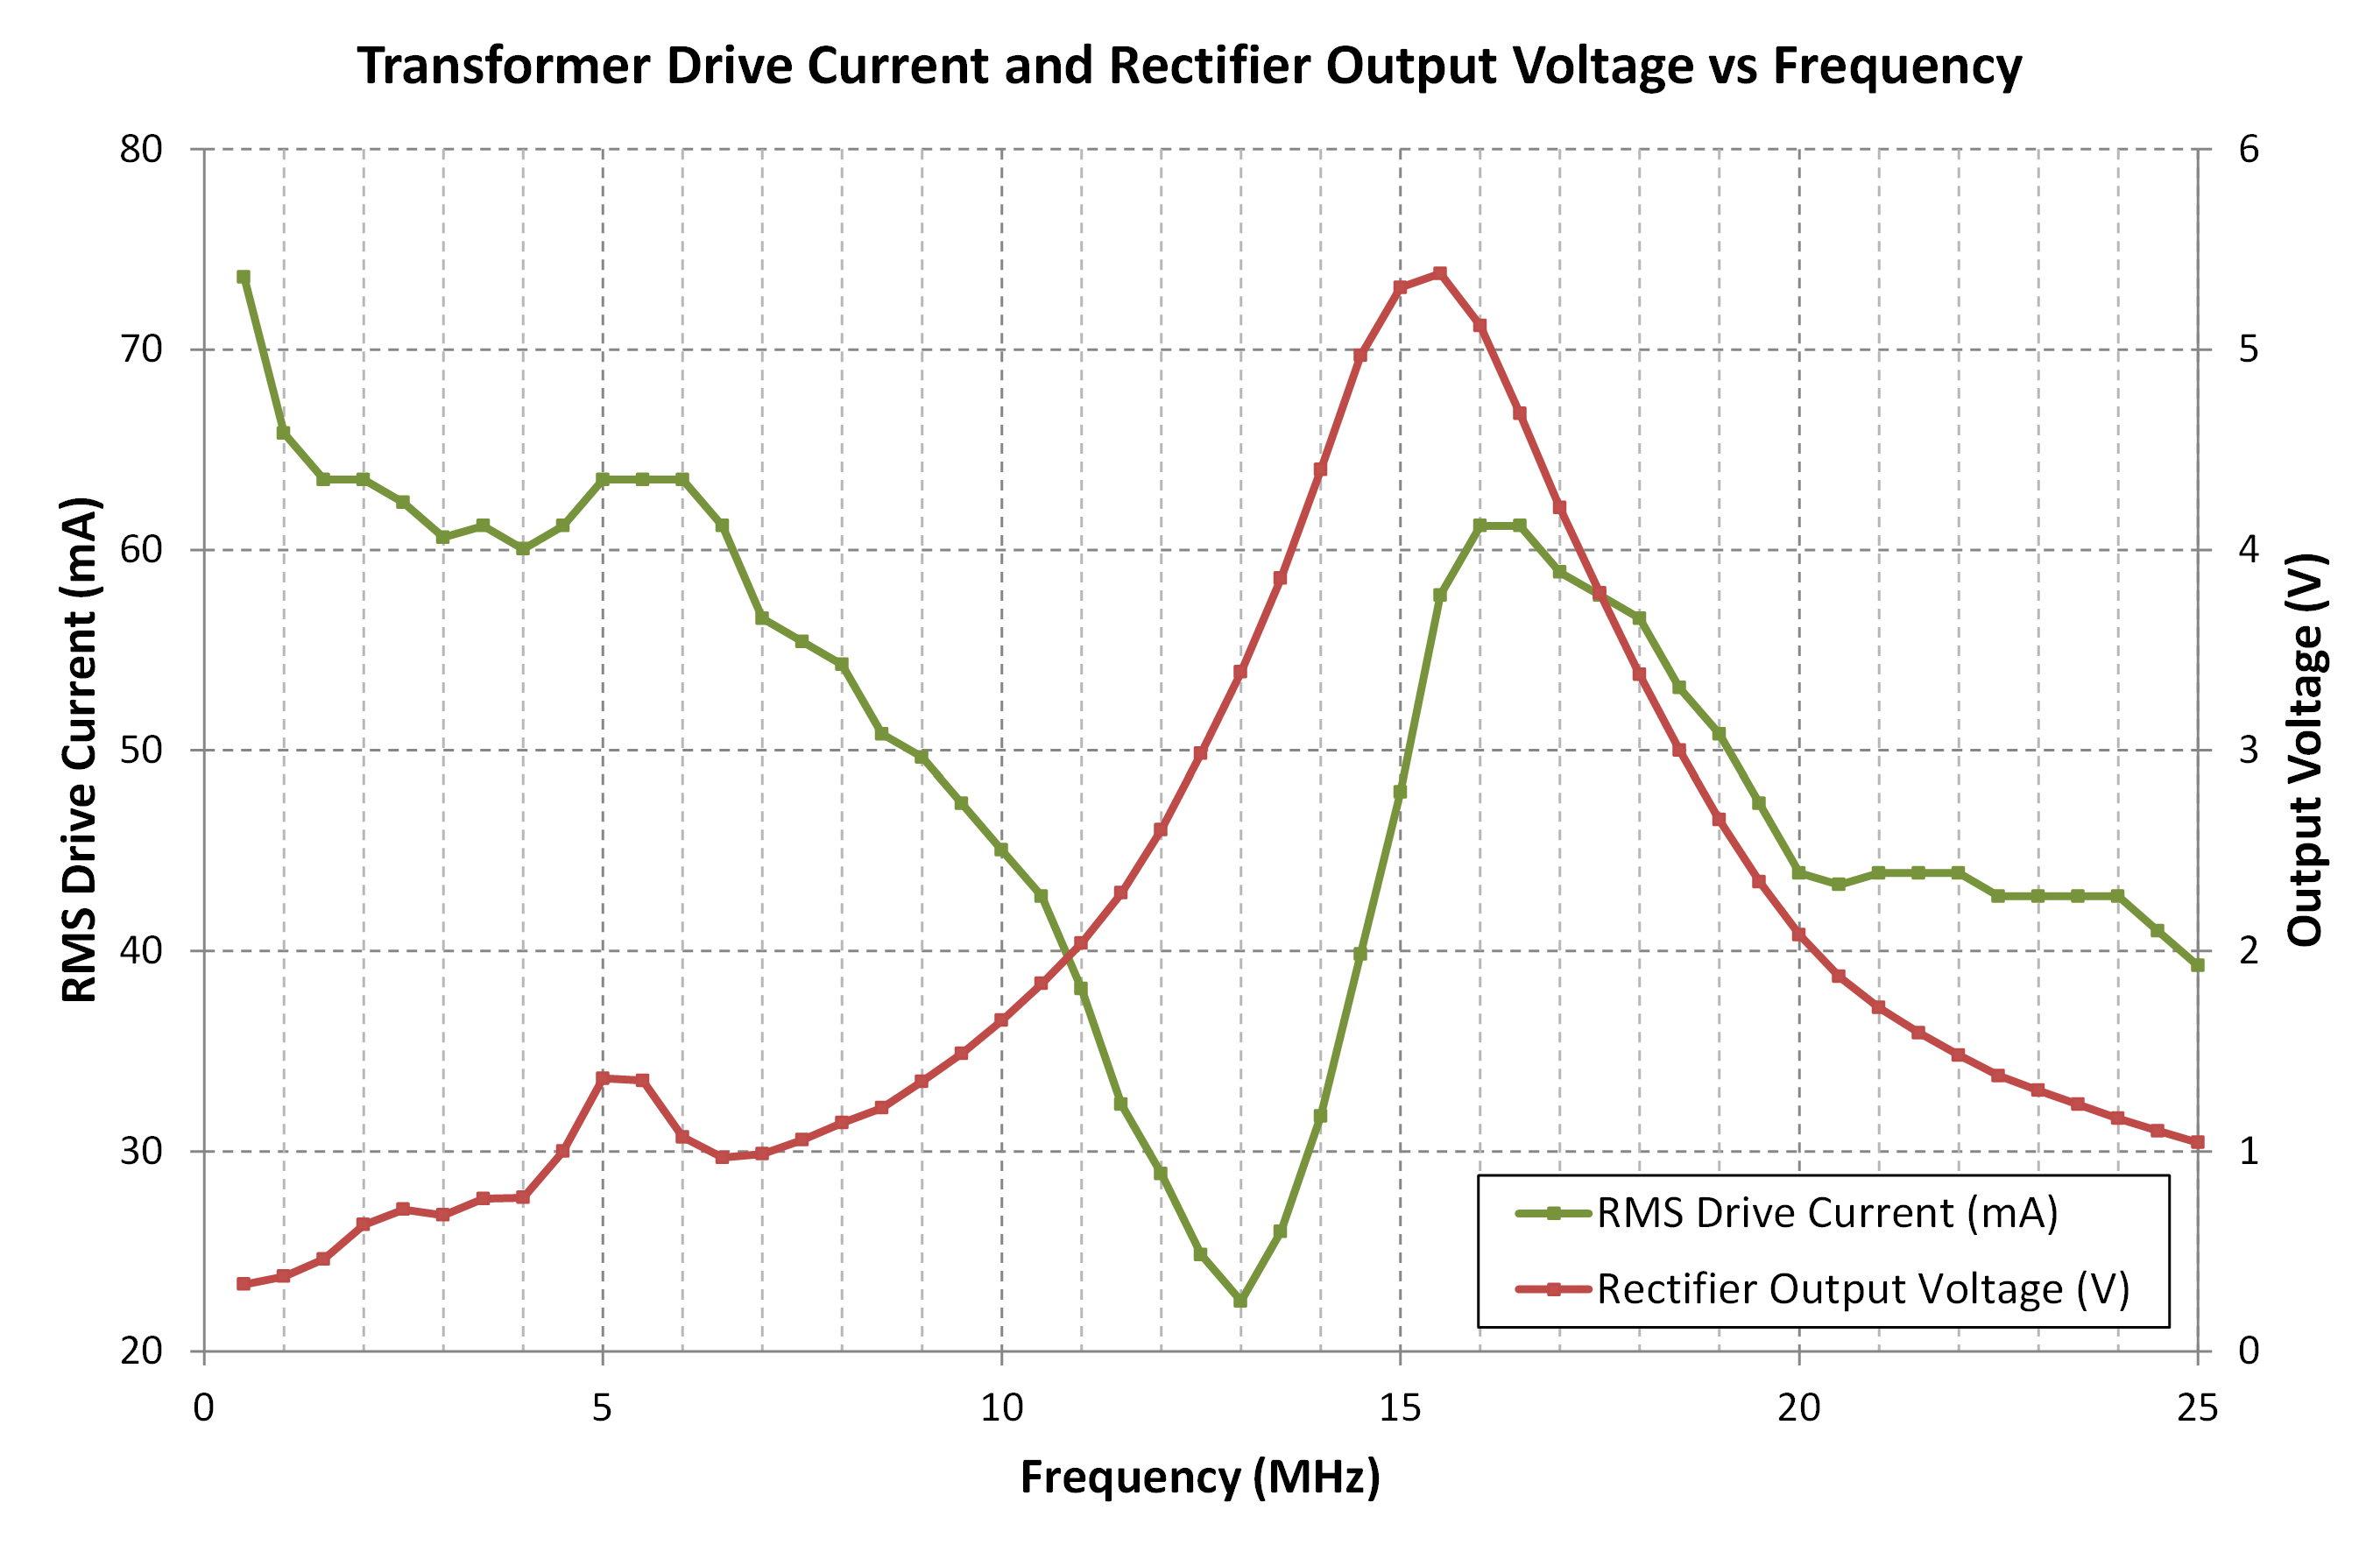
\includegraphics[width=1\columnwidth]{./img/ZandVoutVsF_3V3}
		\caption{Input impedance and output voltage versus frequency at 3.3V.}
		\label{fig:ZandVvsF}
	\end{figure}
	
	\begin{figure}[t]
		\centering
		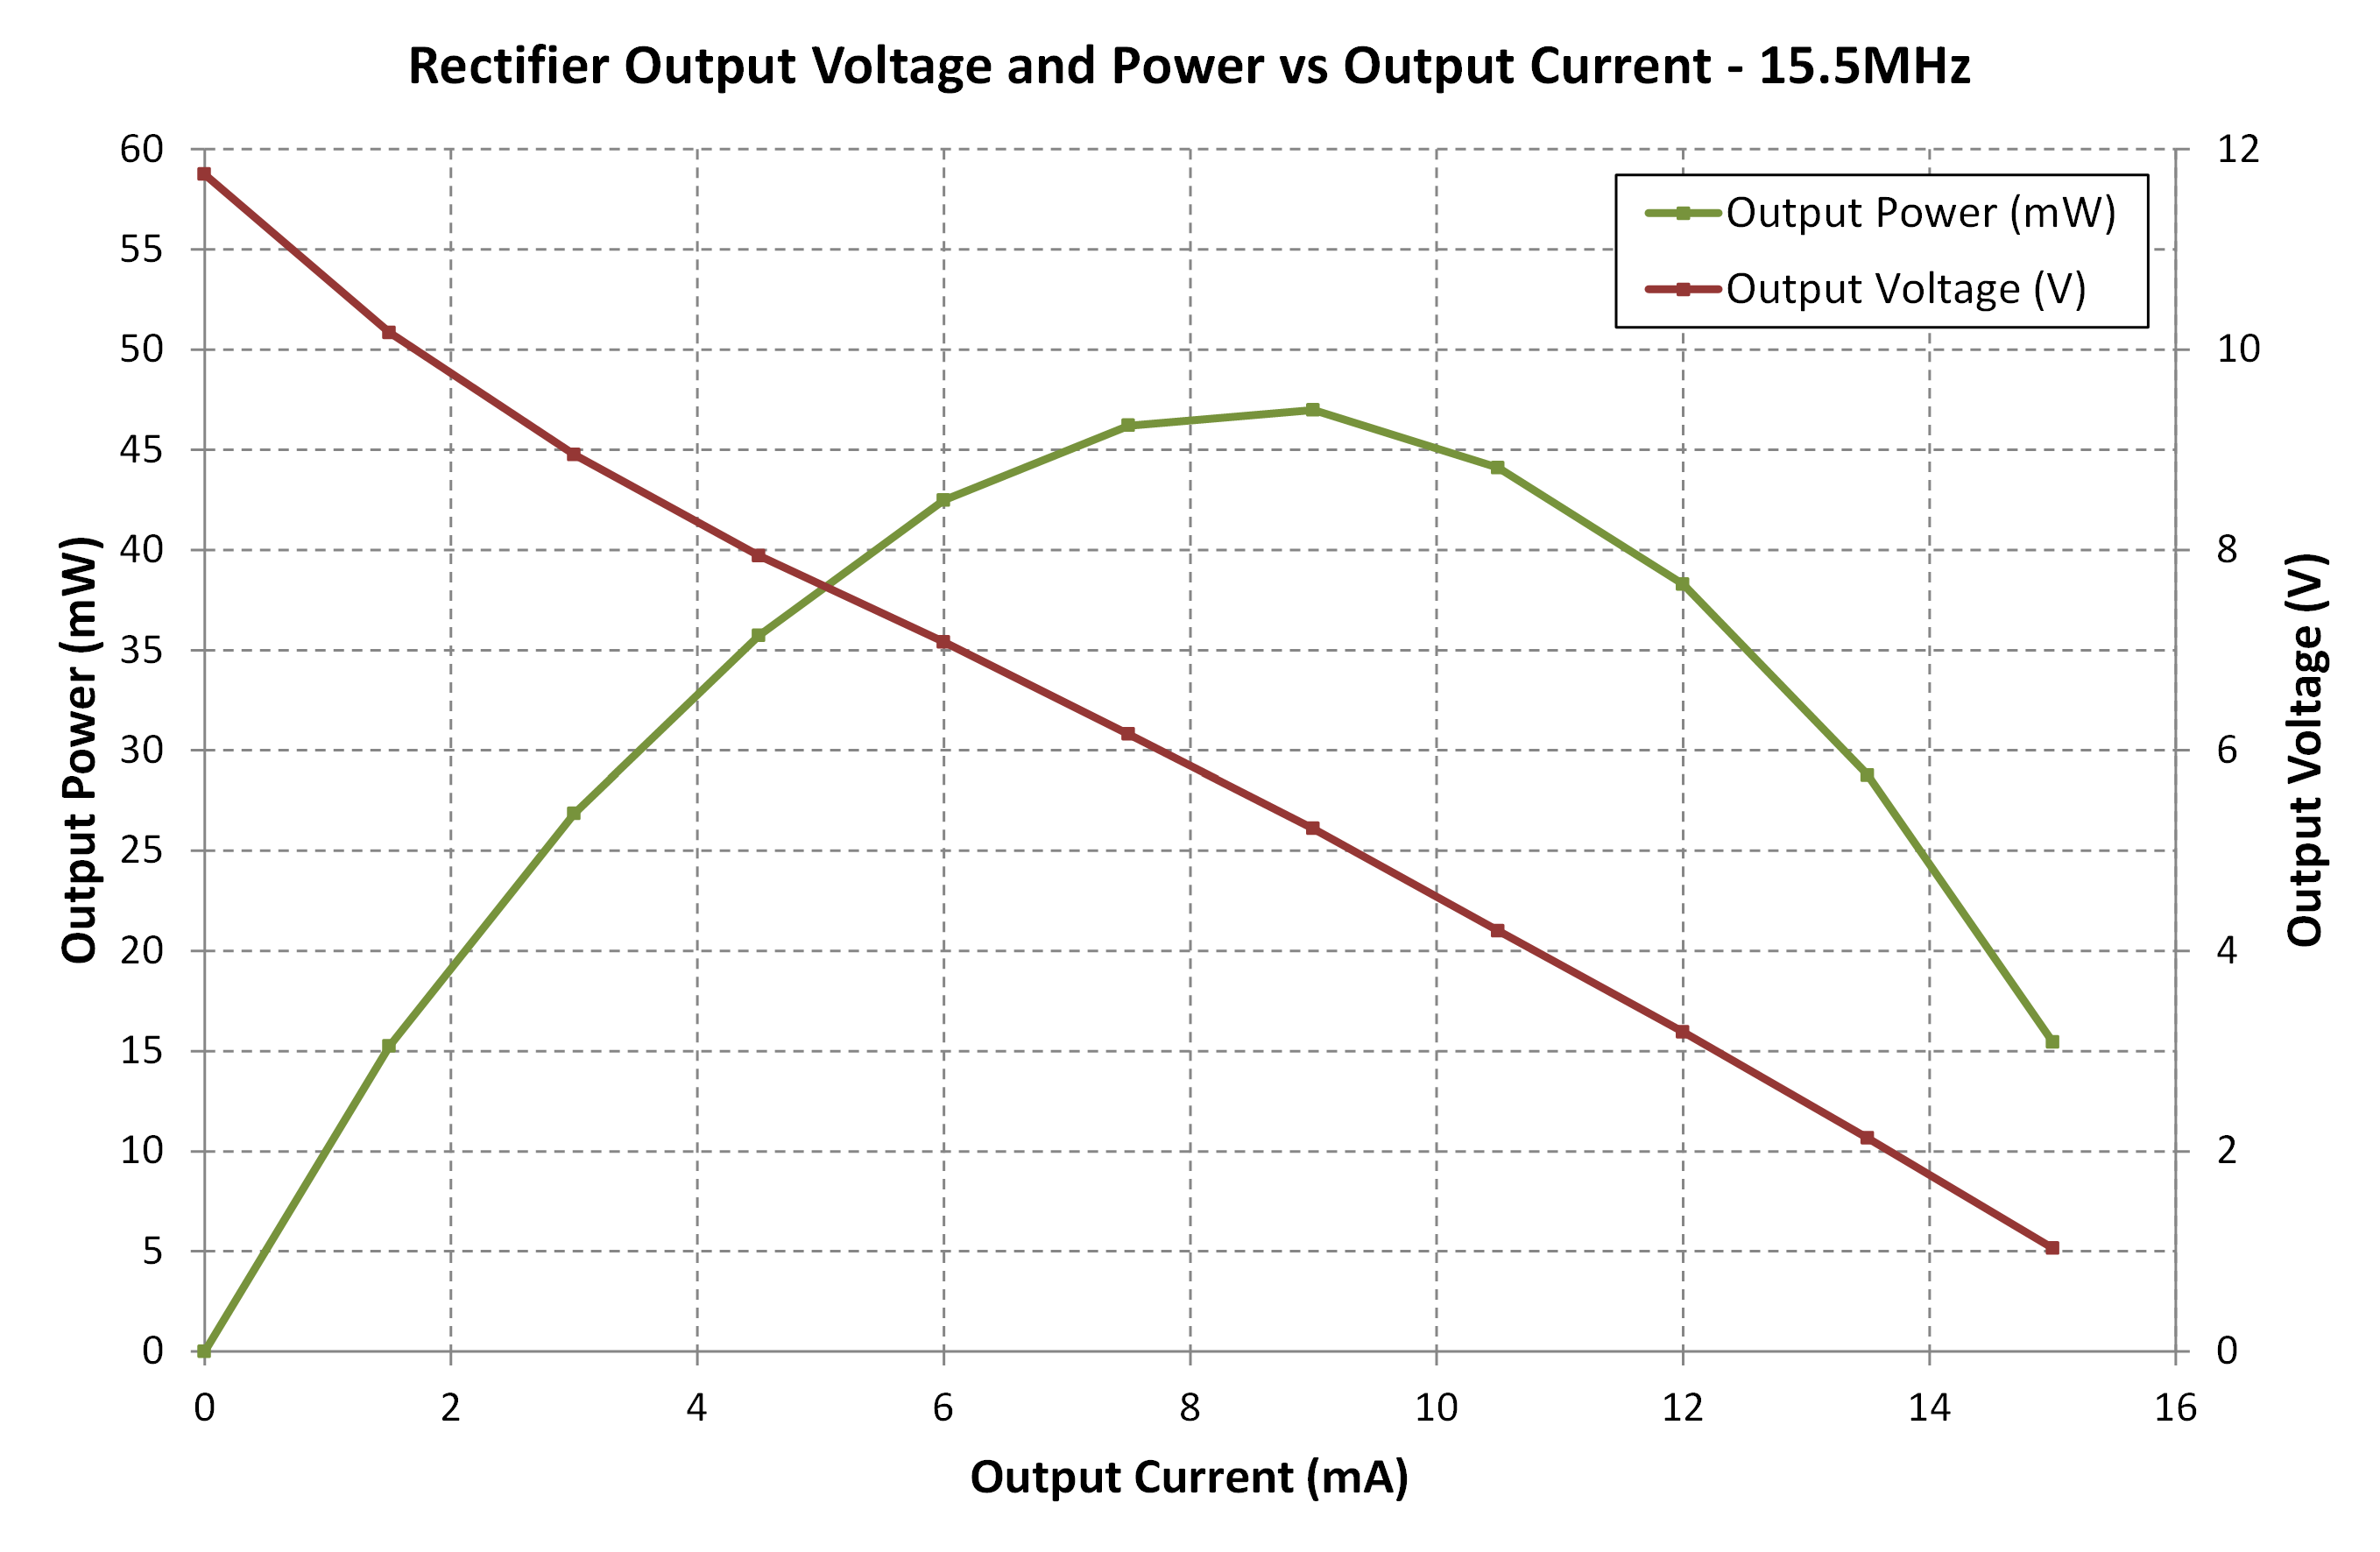
\includegraphics[width=1\columnwidth]{./img/VandPvsI}
		\caption{Secondary output voltage and power versus load current at MEF (15.5MHz).}
		\label{fig:VandPvsI}
	\end{figure}
	
	\begin{figure}[t]
		\centering
		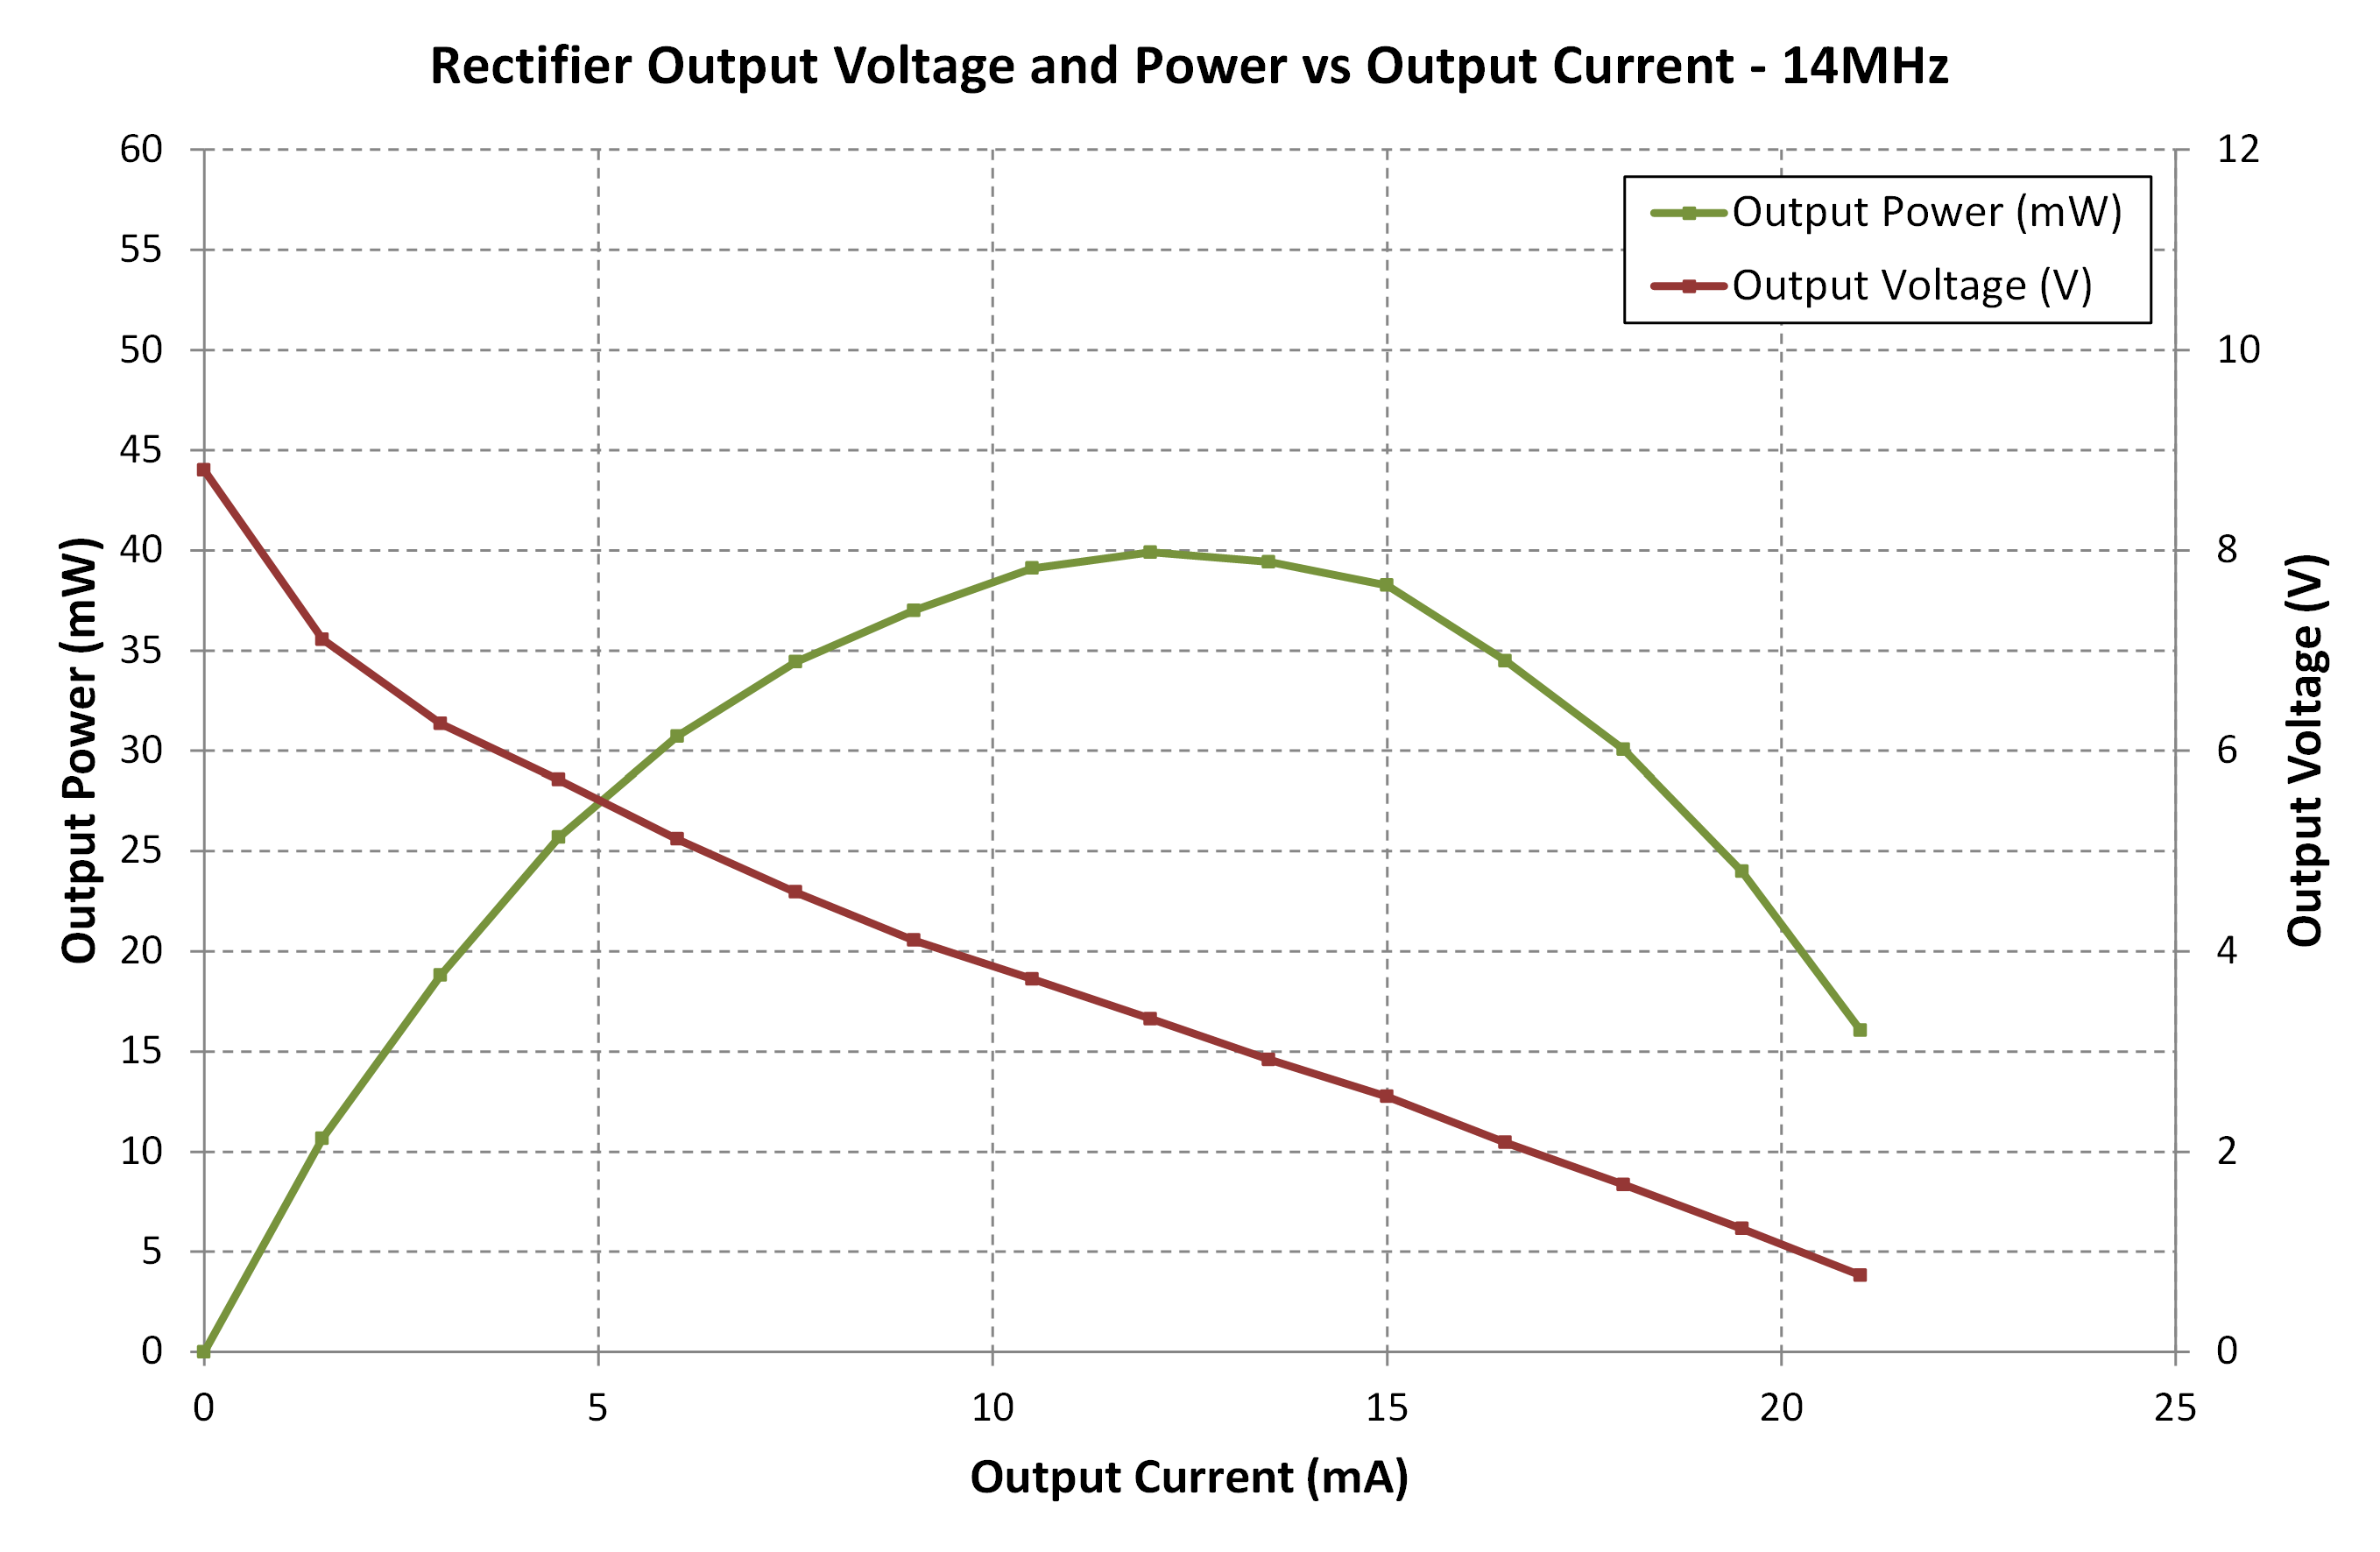
\includegraphics[width=1\columnwidth]{./img/VandPvsI_retuned}
		\caption{Secondary output voltage and power versus load current at MIF-MEF compromise (14MHz).}
		\label{fig:VanndPvsI_retuned}
	\end{figure}
	
	\subsection{Clock generation and recovery}
	Since the sigma-delta modulator's clock is derived from the drive frequency of the primary winding, it is simplest for the primary drive frequency to be an exact power-of-two multiple of the desired modulator frequency, so that a series of D flip-flops may divide the signal down to the desired clock.  Since the test coreless PCB transformer has been designed for a 16MHz resonant frequency (with prior figures showing this to be a good operating point in practice), a single flip flop was used to extract the 8MHz frequency.  Figure \ref{fig:Clock} shows the 16MHz clock signal (Reference - black), secondary output voltage (Channel 1 - blue) and extracted clock signal (Channel 2 - red).  The divide-by-two clock extraction method appears effective, even with a varying secondary load, and further testing showed the simple circuit was able to accurately output a 50\%-duty clock signal over the transformer drive frequency range of 11MHz to 16MHz.  The figures show no reason why a higher order division (divide by 4, for example) could not be used if desired.
	
	\begin{figure}[t]
		\centering
		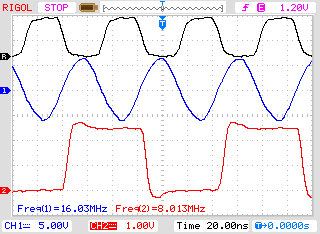
\includegraphics[width=0.8\columnwidth]{./img/Clock}
		\caption{16MHz input clock signal (Reference - black [top]); secondary output voltage (Channel 1 - blue [middle]); 8MHz extracted clock signal (Channel 2 - red [bottom]).}
		\label{fig:Clock}
	\end{figure}
	
	\subsection{Data Recovery}
	% On the data acquisition side of the DAQM, the data transformer winding here is called the primary, and the larger power/clock transformer's winding on this side is called the secondary.  Makes sense from a signal-transfer point of view but could be confusing...
	To test the data recovery circuit, a second PCB transformer was obtained with physical specifications identical to the unit discussed prior.  This second test transformer, however, had its load capacitor (which was 100pF in the prior unit) removed, such that its resonant frequency was much greater than the expected data frequency - a key requirement of the data transfer method.  The decoding circuit was tested by driving the transformer in a single-ended configuration with a simulated data source connected via a small coupling capacitor.  \\
	Since the data recovery circuit was capable of reliable operation with edge spikes of an amplitude as low as about 100mV, the 11-turn transformer was found to be excessive for the data signal transfer scheme.  By cutting the PCB copper tracks on the primary and secondary side of the transformer, the performance of the data recovery circuit was tested for a transformer consisting of five turns and three turns.  The test showed that for a 3.3V square wave input, the five-turn and three-turn transformer yielded edge spikes of amplitude approximately 170mV and 50mV respectively.\\
	Figure \ref{fig:Data} shows the data recovery circuit operating at full-speed (2MHz), where Reference 1 (COLOUR) is the 3.3V, 2MHz simulated data into the 5-turn coreless PCB transformer's primary (which is on the DAQM's acquisition side); Channel 1 (COLOUR) is the voltage at the transformer's secondary (on the DAQM's host-connected side); Channel 2 is the output of the negative edge amplifier (node `Neg Edge' in figure \ref{fig:TFdat}); Channel 3 is the output of the positive edge amplifier (node `Pos Edge' in \ref{fig:TFdat}); and Channel 4 (COLOUR) is the recovered 2MHz data signal. \\
	Testing has demonstrated that the data recovery circuit is effective over a range of data rates and duty cycles, and that a coreless PCB transformer with as few as four to five turns can be expected to yield reliable performance at this data rate.
	
	%MC REMOVED: Due to hardware availability issues, the high-speed ($ t_{d} \leq 10ns $) Schmitt NAND gate specified in the circuit was substituted for an ordinary-speed ($ t_{d} \approx 250ns $) Schmitt NAND gate, which resulted in poor performance above about 500kHz (due to the fast impulses generated by the edge detection circuit).
	% and:
	%  CHANNEL NUMBER in figure \ref{fig:Data} shows the positive and negative edge spikes at the secondary of the five-turn coreless PCB transformer with a 3.3V, 2MHz simulated data signal applied (via a small capacitor).
	%
	% Need to re-test circuit using fast NAND gate on Wed 30th.
	\begin{figure}[t]
		\centering
		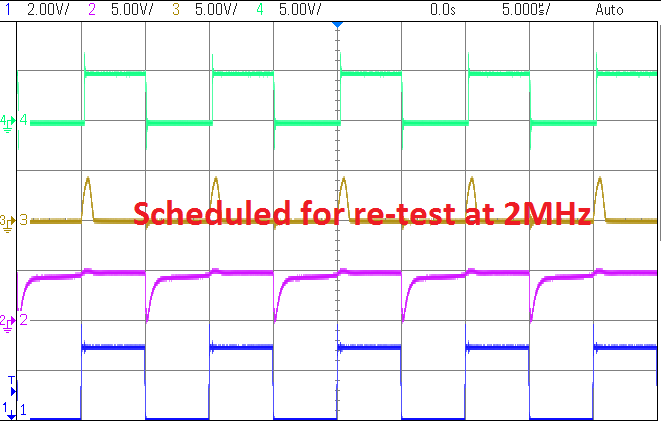
\includegraphics[width=0.8\columnwidth]{./img/DataCroppedREQUPD}
		\caption{Data into transformer (CH1, bottom); output of negative edge amplifier (CH2); output of positive edge amplifier (CH3); recovered data signal at output of transformer (CH4, top).}
		\label{fig:Data}
	\end{figure}

% What this figure shows will soon be presented in figure:Data (above) when it is re-tested
%	\begin{figure}[t]
%		\centering
%		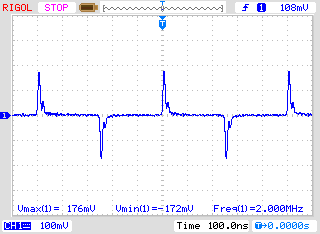
\includegraphics[width=0.8\columnwidth]{./img/5turnTF}
%		\caption{Positive and negative edge spikes at secondary of 5-turn transformer (3.3V primary signal).}
%		\label{fig:5turnTF}
%	\end{figure}

\section{Future work}
% Unsure of my terminology regarding axially and planarly separated.  Meaning:
% Planarly: modules side by side on a flat plane/surface
% Axially: modules stocked on top of each other
The development of the coreless PCB transformer for use in the data acquisition module has yielded two key further research opportunities.  
With each module's coreless PCB transformer operating at 16MHz, significant electromagnetic interference (EMI), both radiated and conducted, may be expected.  Whilst informal experimentation has shown that crosstalk between planarly separated modules (the intended multi-module configuration) is much less than when the modules are axially separated, a thorough analysis has not yet been performed and thus the extent and effect of inter-module interference is not yet known.  \cite{EMIShield} demonstrates that relatively thin (0.4mm) ferrite sheets can provide effective EMI shielding - up to a shielding effectiveness of 40dB for a bare ferrite sheet, or up to 60dB for the same sheet but with copper backing.  Cost analysis has shown that such a ferrite sheet may increase the module cost by 10-20\%, which may represent a worthwhile inclusion.  \\
Other methods for EMI reduction include driving the coreless PCB transformer with a sinusoidal waveform rather than the square waveform used currently, and the possibility of using a spread-spectrum driver in order to reduce the amplitude of the fundamental drive frequency.

The second area of research interest involves the transmission of the 2MHz data signal from the module's secondary side to the primary side, using the same coreless PCB transformer used to transfer the clock signal (16MHz $ \div $ 2 typical) and provide isolated secondary power.  This single-transformer concept is the ultimate goal of the DAQM's coreless PCB transformer design, with the original intention being that the data signal would be load- or resonant frequency-modulated at the secondary, which could be detected by monitoring the transformer's primary-side drive current.  Such disturbance detection is performed in commercial RFID systems, where the receiver modulates its antenna's resonant frequency to allow the transmitter to identify the receiving device \cite{RFID}.  
% MC REmoved:
%In practice, even 100\% load- or resonant frequency-modulation, which also reduces the average output voltage below the minimum requirement, yielded a primary current change of less than ten milliamperes.  This small amplitude distinction, coupled with the limited spectral separation of the data (2MHz) and carrier (16MHz) frequencies, loss of adequate secondary voltage, and the expense of high-speed comparators and op-amps, has proved primary-side data detection to be challenging, particularly with the tight cost constraints imposed by the application.

\section{Conclusion}
The use of planar coreless PCB transformers has received some interest due to the advent of wireless inductive charging systems; however, such transformers have not seen significant use as a power and signal transfer device in commercial electronics.  This paper presented the concept of a isolated, low-cost, modular data acquisition module designed for use in a distributed multi-sensor, single-host environment.  Specifically, planar coreless PCB transformers were introduced and typical design processes and calculations were presented.  The paper experimentally verified the viability of the use of the coreless transformers for the module's isolated power, clock and data signals.  The experimental data presented is considered to be typical of a two-winding coreless PCB transformer, and the calculations and models may be used to represent any such coreless PCB transformer design.  


% conference papers do not normally have an appendix	

% use section* for acknowledgement

% trigger a \newpage just before the given reference
% number - used to balance the columns on the last page
% adjust value as needed - may need to be readjusted if
% the document is modified later
%\IEEEtriggeratref{8}
% The "triggered" command can be changed if desired:
%\IEEEtriggercmd{\enlargethispage{-5in}}

% references section
\bibliographystyle{IEEEtran}
\bibliography{IEEEabrv,references}

\end{document}


